\documentclass[10pt]{article}
\usepackage[utf8]{inputenc}
\usepackage[italian]{babel}
\usepackage{multicol}
\usepackage[a4paper, total={18cm, 25cm}]{geometry}
\usepackage{listings}
\usepackage{graphicx}
\graphicspath{ {./img/} }
\usepackage{color}

\begin{document}
\title{Reti di Calcolatori e Laboratorio}
\author{Federico Matteoni}
\date{ }
\renewcommand*\contentsname{Indice}
\definecolor{pblue}{rgb}{0.13,0.13,1}
\definecolor{pgreen}{rgb}{0,0.5,0}
\definecolor{pred}{rgb}{0.9,0,0}
\definecolor{pgrey}{rgb}{0.46,0.45,0.48}
\lstset{
  language=Java,
  showspaces=false,
  showtabs=false,
  breaklines=true,
  showstringspaces=false,
  breakatwhitespace=true,
  commentstyle=\color{pgreen},
  keywordstyle=\color{pblue},
  stringstyle=\color{pred},
  basicstyle=\small\ttfamily
}

\maketitle
\begin{multicols}{2}
\tableofcontents
\end{multicols}
\pagebreak
\section{Introduzione}
Appunti del corso di \textbf{Reti di Calcolatori} presi a lezione da \textbf{Federico Matteoni}.\\\\
Prof.: \textbf{Federica Paganelli}, federica.paganelli@unipi.it\\
\begin{list}{-}{Riferimenti web:}
\item \emph{elearning.di.unipi.it/enrol/index.php?id=169}\\Password: \textbf{RETI2019}
\end{list}
Esame: scritto (o compitini), discussione orale facoltativa + progetto con discussione (progetto + teoria di laboratorio, progetto da consegnare 7gg prima della discussione)\\
\begin{list}{-}{Libri e materiale didattico:}
\item Slide su eLearning
\item IETF RFC\\tools.ietf.org/rfc\\www.ietf.org/rfc.html
\item "Computer Networks: A Top-Down Approach" B. A. Forouzan, F. Mosharraf, McGraw Hill
\end{list}
Ricevimento: stanza 355 DO, II piano

\section{Rete}
\paragraph{Definizione di rete} Interconnessione di dispositivi in grado di scambiarsi informazioni, come end system, router, switch e modem.\\
\begin{list}{}{Gli end system possono essere di due tipi:}
\item \textbf{Host}: una macchina, in genere di proprietà degli utenti, \textbf{dedicata ad eseguire applicazioni}. Esempi: desktop, portatile, smartphone, tablet\ldots
\item \textbf{Server}: una macchina, tipicamente con elevate prestazioni, destinata ad eseguire programmi che \textbf{forniscono servizi} a diverse applicazioni utente. Esempi: posta elettronica, web, \ldots
\end{list}
\textbf{Con il termine host si può anche indicare un server}.

\subsection{Tipi di Rete}
\paragraph{Local Area Network} Una \textbf{LAN è una rete di area geografica limitata}: un ufficio, una casa ecc.. I dispositivi comunicano attraverso una determinata tecnologica: switch, BUS, HUB ecc..\\
In una rete locale tipicamente una serie di host comunicano tra loro attraverso, ad esempio, uno switch centrale.
\paragraph{Wide Area Network} Alcuni esempi:\\
\begin{multicols}{2}
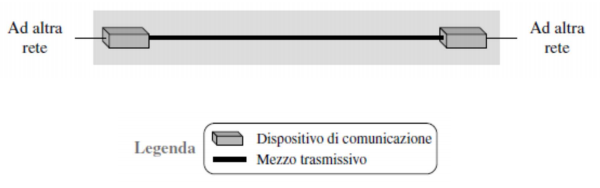
\includegraphics[scale=0.5]{wan1.png}\\
\columnbreak
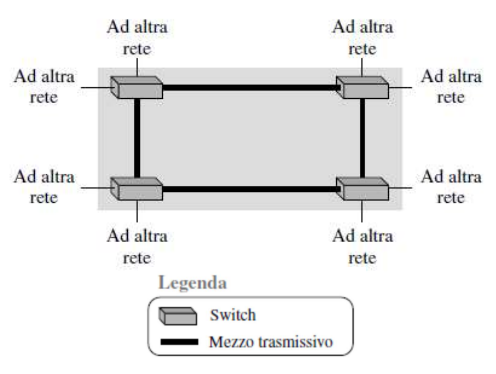
\includegraphics[scale=0.5]{wan2.png}\\
\end{multicols}

\subsection{Internetwork}
Una \textbf{internetwork} si crea quando si \textbf{interconnettono diverse reti}.
Alcuni esempi:\\
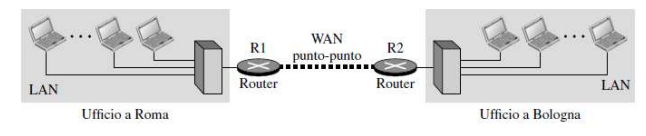
\includegraphics[scale=1]{internetwork1.png}\\
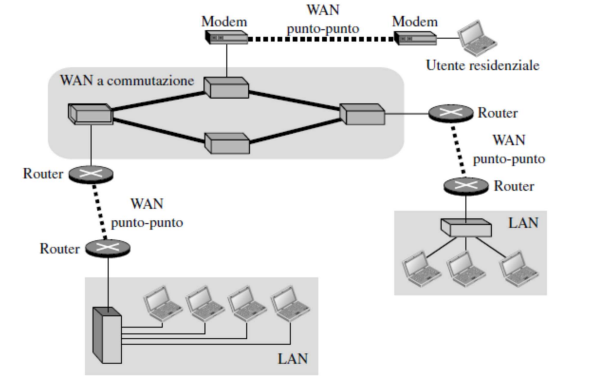
\includegraphics[scale=0.75]{internetwork2.png}\\

\subsection{Switching}
Una rete internet è formata dall'interconnesione di reti composte da link e dispositivi capaci di scambiarsi informazioni.
In particolare, i sistemi terminali comunicano tra di loro per mezzo di dispositivi come switch, router ecc. che si trovano nel percorso tra i sistemi sorgente e destinazione.
\paragraph{Switched Network} Reti a commutazione di circuito, tipico delle vecchie reti telefoniche\\
Le risorse sono riservate end-to-end per una connessione. Le risorse di rete (es. bandwidth) vengono suddivise in pezzi, e ciascun pezzo è allocato ai vari collegamenti. Le risorse rimangono inattive se non vengono utilizzate, cioè \textbf{non c'è condivisione}. L'allocazione della rete rende necessario un setup della comunicazione.\\A tutti gli effetti vi è un circuito dedicato per tutta la durata della connessione. Ciò è rende poco flessibile l'utilizzo delle risorse (\textbf{overprovisioning}).
\paragraph{Packet-Switched Network} Reti a commutazione di pacchetto, più moderno\\
Flusso di dati punto-punto suddiviso in pacchetti. I pacchetti degli utenti condividono le risorse di rete. Ciascun pacchetto utilizza completamente il canale.\\\textbf{Store and Forward}: il commutatore deve ricevere l'intero pacchetto prima di ritrasmetterlo in uscita.\\Le risorse vengono usate \textbf{a seconda delle necessità}. Vi è \textbf{contesa per le risorse}: la richiesta di risorse può eccedere la disponibilità e si può verificare \textbf{congestione} quando i pacchetti vengono accodati in attesa di utilizzare il collegamento. Si possono anche verificare perdite.
\section{Internet} L'internetwork più famosa ed utilizzata è \textbf{internet}, ed è composta da migliaia di reti interconnesse. \textbf{Ogni rete} connessa ad internet \textbf{deve utilizzare il protocollo IP} e rispettare certe convenzioni su nomi ed indirizzi. Si possono aggiungere nuove reti ad internet molto facilmente.
\paragraph{Dispositivi in internet} I \textbf{dispositivi} connessi ad internet possono essere host, end systems come PC, workstations, servers, pda, smartphones ecc\ldots\\
I \textbf{link di comunicazione} possono essere fibre ottiche, doppini telefonici, cavi coassiali, onde radio\ldots
Le \textbf{entità software} in internet possono essere:
\begin{list}{}{}
\item \textbf{Applicazioni} e processi
\item \textbf{Protocolli}: regolamentano la trasmissione e la ricezione di messaggi (TCP, IP, HTTP, FTP, PPP\ldots)
\item \textbf{Interfacce}
\item \textbf{Standard} di internet e del web: RFC (Request for Comments) e W3C.
\end{list}
\textbf{Internet è una visione dei servizi}. L'infrastruttura di comunicazione permette alle applicazioni distribuite di scambiare informazioni (WWW, e-mail, giochi, e-commerce, controllo remoto\ldots) e fornisce loro \textbf{servizi di comunicazione connectionless} (senza garanzia di consegna) o \textbf{connection-oriented} (dati garantiti in integrità, completezza ed ordine).
\subsection{Enti Ufficiali} L'\textbf{Internet Engineering Task Force} (IETF) è l'organismo che studia e sviluppa i protocolli in uso su internet. Si basa su gruppi di lavoro a cui chiunque può accedere. I documenti ufficiali che pubblica, dove descrivono i protocolli usati in internet, sono gli RFC/STD (Request for Comments/STanDards).\\
L'\textbf{Internet Corporation for Assigned Names and Numbers} (ICANN) si occupa di coordinare il sistema dei \textbf{nomi di dominio} (DNS) e assegna i gruppi di indirizzi, gli identificativi di protocollo.\\\\
\begin{center}
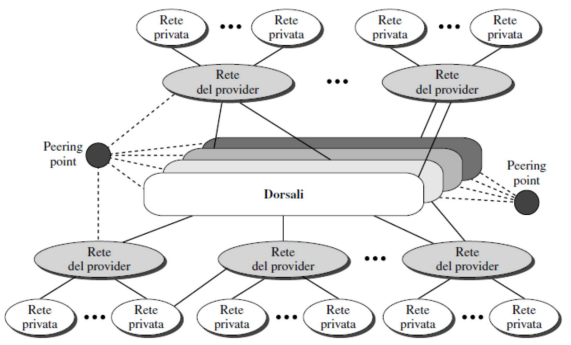
\includegraphics[scale=1]{internet.png}\\
\textbf{Peering point}: interconnessione tra due sistemi autonomi\\
\end{center}
\pagebreak
\subsection{Reti di accesso} Il collegamento tra l'utente ed il primo router di internet è detto \textbf{rete di accesso}.
\begin{list}{}{Può avvenire in 3 modi:}
\item \textbf{Tramite rete telefonica}: servizio dial-up, ADSL\ldots
\item \textbf{Tramite reti wireless}
\item \textbf{Collegamento diretto}, come collegamenti WAN dedicati ad alta velocità (aziende e università)
\end{list}
\section{Metriche di Riferimento}
Come misurare le prestazioni della rete?
\begin{list}{}{Tramite una serie di metriche:}
\item \textbf{Bandwith} o ampiezza di banda: è la larghezza dell'intervallo di frequenze utilizzato dal sistema trasmissivo (Hz).\\\textbf{Bitrate} o \textbf{transmission rate}: quantità di bit che possono essere trasmessi o ricevuti nell'unità di tempo (bit/secondo, bps)\\Il bitrate dipende dalla bandwidth e dalla tecnica trasmissiva utilizzata.
\item \textbf{Throughput}: la quantità di traffico che arriva realmente a destinazione nell'unità di tempo (al netto di perdite sulla rete, funzionamento dei protocolli ecc\ldots).\\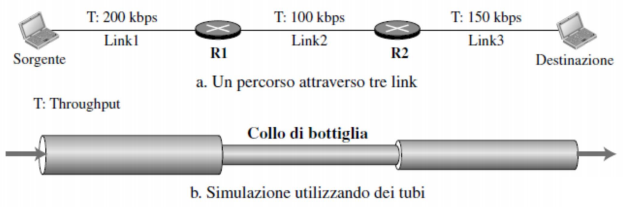
\includegraphics[scale=1]{throughput.png}\\Non è detto che corrisponda alla bandwidth perché ci potrebbe essere un collo di bottiglia.
\item \textbf{Latenza} o ritardo: il tempo richiesto affinché un messaggio arrivi a destinazione dal momento in cui il primo bit parte dalla sorgente.\\
\texttt{latenza = ritardo di propagazione + ritardo di trasmissione + ritardo di accodamento + ritardo di elaborazione}
\item \textbf{Perdita di pacchetti}. Come si può verificare?\\
\begin{multicols}{2}
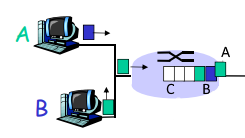
\includegraphics[scale=1]{ritpackets.png}\\

\columnbreak
A $\rightarrow$ pacchetti \textbf{in attesa} di essere trasmessi (\emph{ritardo})\\
B $\rightarrow$ pacchetti \textbf{accodati} (\emph{ritardo})\\
C $\rightarrow$ buffer \textbf{liberi} (se non ci sono buffer liberi, i pacchetti in arrivo vengono scartati, \emph{perdita})\\\\
I pacchetti da spedire vengono accodati nei buffer dei router. Di solito, il tasso di arrivo dei pacchetti sul router eccede le capacità del router di evaderli, quindi \textbf{i pacchetti si accodano in attesa del proprio turno}.
\end{multicols}
Il \textbf{ritardo di elaborazione} è dato dal controllo sui bit e dalla determinazione del canale di uscita (trascurabile)\\
Il \textbf{ritardo di accodamento} è dato dall'attesa di un pacchetto di essere trasmesso (B)\\
Il \textbf{ritardo di trasmissione} è il tempo impiegato per trasmettere un pacchetto sul link.\\\texttt{R$_{trasmissione}$ = R/L}\\
\texttt{R} = rate di trasmissione del collegamento, in bps\\
\texttt{L} = lunghezza del pacchetto in bit\\
Il \textbf{ritardo di propagazione} è il tempo impiegato da 1 bit per essere propagato da un nodo all'altro.\\\texttt{R$_{propagazione}$ = d/s}\\
\texttt{d} = lunghezza del collegamento\\
\texttt{s} = velocità di propagazione del collegamento (si usa la velocità della luce, circa 3 x 10$^{8}$ m/s)
\end{list}
\texttt{d$_{nodal}$ = d$_{proc}$ + d$_{queue}$ + d$_{trans}$ + d$_{prop}$}\\
\texttt{d$_{proc}$} = \textbf{ritardo di elaborazione}, pochi microsecondi\\
\texttt{d$_{queue}$} = \textbf{ritardo di accodamento}, dipende dalla congestione\\
\texttt{d$_{trans}$} = \textbf{ritardo di trasmissione}, \texttt{L/R} e significativo a lunga distanza\\
\texttt{d$_{prop}$} = \textbf{ritardo di propagazione}, \texttt{d/s}, da pochi microsecondi a centinaia di millisecondi\\
\section{Modelli Stratificati}
$https://elearning.di.unipi.it/pluginfile.php/27387/mod_resource/content/1/L02_introduzione_protocolli.pdf$
\paragraph{Perché usare un modello a strati} Per mandare dei dati da un host ad un altro comunicando su una rete, si devono eseguire una \textbf{serie di operazioni}: \textbf{trovare il percorso} di rete da attraversare, \textbf{decidere in che modo spedire e codificare} i dati, \textbf{risolvere eventuali problemi} di comunicazione e altro ancora.\\
Programmare ogni volta tutto il procedimento è un \textbf{lavoro estremamente complesso} e ripetitivo. Un modello a strati \textbf{astrae su più livelli il problema della trasmissione dati} in modo da fornire di volta in volta strumenti utili al programmatore per poter evitare di "\textit{reinventare la ruota}".
\paragraph{Definizioni generali} Nelle architetture di comunicazione a strati sono importanti una serie di definizioni:
\begin{list}{-}{}
\item Stratificazione
\item Information hiding
\item Separation of concern
\item Modello ISO/OSI
\item Stack TCP/IP
\end{list}
Tali definizioni verranno viste durante il corso.
\paragraph{Lo Strato} Uno \textbf{strato} è un \textbf{modulo interamente definito} attraverso i servizi, le interfacce e i protocolli che lo caratterizzano. Si indica anche col nome di livello.\\
Uno strato \texttt{n} \textbf{comunica direttamente} con lo strato \texttt{n} di un'altra unità tramite un \textbf{protocollo assegnato}. Lo stesso strato \texttt{n} può richiedere servizi allo strato \texttt{n-1} attraverso la \textbf{loro interfaccia}, e fornisce servizi allo strato \texttt{n+1} attraverso la \textbf{rispettiva interfaccia}.
\paragraph{Es. modello stratificato: sistema postale}\texttt{Vedi slide\\$https://elearning.di.unipi.it/pluginfile.php/27387/mod_resource/content/1/L02_introduzione_protocolli.pdf$, 48}\\
Dal livello più alto al livello più basso per la spedizione, viceversa per la ricezione. Un problema importante che si incontra quando si manda una lettera, ad esempio, dall'Italia al Giappone è la traduzione. In una \textbf{serie di passi}, in cui in ognuno viene \textbf{eseguito un particolare compito su un messaggio}, che viene poi \textbf{trasferito ad un altro livello}. Nell'esempio, la segretaria prepara lettera (traduce in giapponese e imbusta) affinché il postino la possa prendere. Però il "messaggio" della segretaria è "scritto" per essere interpretato dalla segretaria giapponese, il direttore italiano scrive per il direttore giapponese. \textbf{Messaggi di un livello del sistema che spedisce sono scritti per essere interpretati dal medesimo livello del sistema ricevente}.
\subsection{Perché stratificare} La stratificazione è molto utile per \textbf{scomporre il sistema complesso della gestione della comunicazione}. Prendo un sistema estremamente costoso da costruire per una singola coppia di aziende, quindi lo trasformo in strati così che il costo della singola lettera sia irrisorio.\\
\textbf{Definisco funzioni di base per effettuare trasferimento e agenti che le svolgono}.
\begin{list}{}{Principi di base:}
\item \textbf{Separation of Concern}\\\textbf{Far fare} ad un determinato strato \textbf{solo ciò che gli compete}, \textbf{delegando agli altri tutto ciò che è delegabile}
\item \textbf{Information Hiding}\\\textbf{Nascondo} ad un determinato strato \textbf{le informazioni non indispensabili allo svolgere della sua operazione}.
\end{list}

\paragraph{Esempio} Se traduco il modello postale nel modello a strati ho, ad esempio:\\
\begin{center}
\begin{multicols}{2}
Utente\\Segretaria\\Postino\\Smistamento\\Stazione\\
\columnbreak
Utente\\Segretaria\\Postino\\Smistamento\\Stazione\\
\end{multicols}
---Viaggio$\rightarrow$
\end{center}

\subsection{Smistamento Intermedio} Spedire un pacchetto che è destinato ad determinato livello intermedio. Quindi \textbf{arrivo fino al corrispondente livello intermedio per evitare che si possano esporre info sensibili}.
\subsection{Elementi fondamentali}
Gli \textbf{elementi fondamentali} del modello stratificato sono:
\begin{list}{}{}
\item Flusso dati
\item \textbf{Servizio}: una \textbf{funzione} che uno strato offre allo strato superiore, attraverso un'interfaccia.
\item Protocollo
\item \textbf{Interfaccia}: \textbf{insieme di regole} che governano il formato e il significato dei frame, pacchetti o messaggi che vengono \textbf{scambiati tra strati adiacenti della stessa entità}.
\end{list}
\textbf{I servizi indicano \textit{cosa} si può fare, le interfaccie regolano \textit{come} si può fare.}

\subsection{Modalità di Servizio}
\begin{list}{}{I \textbf{dati} possono essere scambiati in due modalità diverse:}
\item \textbf{Connection-Oriented}: il livello di trasferimento stabilisce una \textbf{connessione logica} tra due sistemi.
\begin{list}{--}{La connessione è quindi \textbf{gestita}:}
\item \textbf{Instaurazione} della connessione
\item \textbf{Trasferimento} dei dati
\item \textbf{Chiusura} della connessione
\end{list}
\item \textbf{Connectionless}: i dati vengono \textbf{trasferiti senza stabilire una connessione}.
\end{list}
\subsection{Vantaggi}
Il vantaggio più grosso è che \textbf{sviluppare il singolo strato è più semplice ed economico rispetto a sviluppare tutto il sistema complesso}. Questo perché \textbf{i servizi degli strati inferiori vengono usati da più entità che implementano gli strati superiori}.
\pagebreak
\section{Protocolli}
\paragraph{Cos'è un protocollo} Un \textbf{protocollo} è un \textbf{insieme di regole} che dice come comunicare ed esporre dati verso l'esterno. I protocolli \textbf{definiscono il formato e l'ordine dei messaggi inviati e ricevuti, con le azioni per trasmette e ricevere tali messaggi}.
\subsection{Incapsulamento} Processo in cui \textbf{aggiungo strati, "involucri" al messaggio originale che vengono man mano tolti alla destinazione}.
\section{OSI RM (Open Systems Interconnction Reference Model)}
Le prime reti erano chiuse, composte da tecnologie e protocolli proprietari. Alcuni esempi sono ARPANET, SNA (IBM), DNA (Digital). Non potevano intercomunicare tra loro, perché usavano \textbf{protocolli diversi}, erano costruite per servizi specifici (TELCO). Insorse quindi un obiettivo: creare un \textbf{modello di riferimento per sistemi aperti}, per permettere a qualsiasi terminale di poter comunicare mediante qualsiasi rete. C'era quindi necessità di \textbf{accordarsi sulle regole}.
\paragraph{OSI} L'OSI è una \textbf{collezione di protocolli aperti}: questo significa che i loro \textbf{dettagli sono pubblici} e i \textbf{cambiamenti vengono gestiti da un'organizzazione con partecipazione aperta al pubblico}. \textbf{Un sistema che implementa i protocolli aperti è un sistema aperto}.
\subsubsection{Pila di protocolli} L'\textbf{OSI} prevede \textbf{sette strati di protocolli}: 
\begin{list}{}{}
\item\textbf{7. Applicativo}: elaborazione dei dati
\item\textbf{6. Presentazione}: unificazione dei dati, preparazione del \textbf{pacchetto} da trasmettere/ricevere
\item\textbf{5. Sessione}:  controllo del dialogo tra gli host sorgente e destinazione.
\item\textbf{4. Trasporto}: offre il vero e proprio trasferimento dati tra gli host terminali, cioè \textbf{astrae la logica} con la quale si scambiano i dati tra host e gestisce gli errori. Realizza il \textbf{dialogo end-to-end}.
\item\textbf{3. Rete}: instradamento del traffico (principalmente router, offre il servizio di consegna attraverso il sistema distribuito dei nodi intermedi).
\item\textbf{2. Datalink}: consegna il frame tra le interfacce, interpretato dalla scheda di rete.
\item\textbf{1. Fisico}: modulazione del segnale elettrico per trasmettere correttamente il flusso di bit sul mezzo fisico.
\end{list}
I livelli \textbf{7-5} si possono raggruppare in più modi, principalmente sono gli strati di supporto all'elaborazione e all'interazione con l'utente. Sono livelli \textbf{software}\\
I livelli \textbf{4-1} sono \textbf{software e hardware}. Sono strati di supporto alla rete e all'infrastruttura trasmissiva, cioè gestiscono la vera e propria trasmissione dei dati.
\pagebreak
\section{Flusso dell'Informazione}
Per le reti, l'informazione ha origine al \textbf{livello applicativo}, che la genera per mandarla in remoto. Una volta generata, essa discende i vari livelli fino al canale fisico e ogni livello \textbf{aggiunge} all'informazione ricevuta dal livello superiore \textbf{una -- o più -- propria sezione informativa} sotto forma di \textbf{header}, contenente informazioni esclusive di quel livello. Per l'informazione ricevuta, si segue il \textbf{cammino inverso}, quindi dal basso verso il livello applicativo, e ogni livello "spacchetta" l'header del livello corrispondente, ne legge le informazioni esclusive e lo gestisce appositamente.\\Il \textbf{processo di incapsulamento} è quindi \textbf{reversibile}: ogni livello esegue una operazione di incapsulamento su dati già incapsulati dal livello precedente, in modo tale da garantire la possibilità di estrarre i dati precedentemente incapsulati.\\
\
\begin{center}
\rule{6.8cm}{1pt}\\
HEADER ||| DATA ||| TRAILER\\
\rule{6.8cm}{1pt}\\
\end{center}
\textbf{Header}: qualificazione del pacchetto per questo livello\\
\textbf{Data}: payload proveniente dal livello superiore\\
\textbf{Trailer}: generalmente usato in funzione del trattamento dell'errore\\
\begin{center}
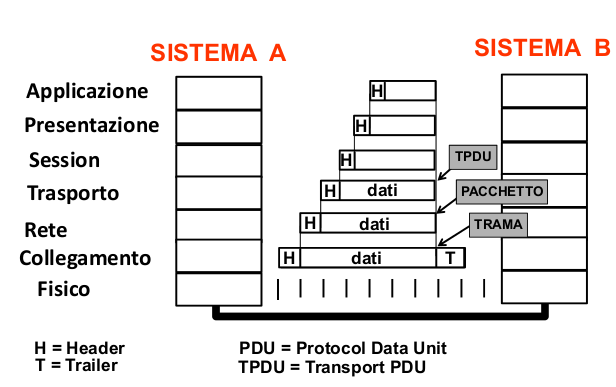
\includegraphics[scale=0.75]{incapsulamento.png}
\end{center}
\pagebreak
\section{Stack protocollare TCP/IP}
Il \textbf{TCP/IP} è una famiglia di protocolli attualmente utilizzati in internet. Si tratta di una \textbf{gerarchia di protocolli} costituita da \textbf{moduli interagenti}, ciascuno con funzioni specifiche.
\paragraph{Gerarchia} Con il termine \textbf{gerarchia} s'intende che ciascun protocollo di livello superiore è \textbf{supportato dai servizi forniti dai protocolli di livello inferiore}. Cioè un protocollo a livello \texttt{n} realizza le sue funzionalità grazie ai protocolli a livello \texttt{n-1}.
\begin{multicols}{2}
\subsection{I Livelli}
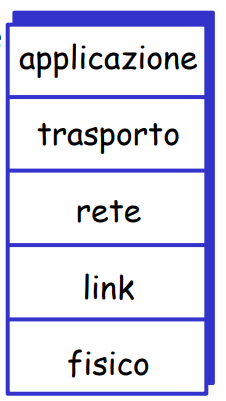
\includegraphics[scale=0.8]{stacktcpip.png}
\columnbreak


Lo stack TCP/IP in origine era intesa come \textbf{quattro livelli software} sovrastanti \textbf{un livello hardware}. Oggi è intesa come semplicemente \textbf{composta da 5 livelli}
\paragraph{Livello Applicativo} Il livello più alto, con il quale interagisce l'utente\\
Identificativi risorse: URL, URI, URN\\
Il web: user agents, http: request, response, connessioni persistenti, GET, POST, PUT, DELETE, status code, proxy server, caching\\
FTP: connessioni dati e di controllo, rappresentazione\\
TELNET\\
Posta elettronica: SMTP, POP3, IMAP\\
DNS e risoluzioni nomi: gerarchia nomi, risoluzione iterativa e ricorsiva, formato pessaggi, nslookup...
\paragraph{Livello Trasporto} Livello al quale si definisce la codifica e il protocollo di trasporto\\
Servizi: mux demux, controllo errore, connectionless\\
TCP: formato segmenti, gestione connessione, controllo flusso e congestione\\
UDP: formato segmenti
\paragraph{Livello Rete} Dove si gestisce l'indirizzamento dei vari host\\
Strato di rete e funzioni\\
Indirizzamentoi IP: classful IPv4, NAT, sottoreti e maschere, classless, CIDR\\
Risoluzione IP e MAC, ARP\\
IPv4: formato datagramma ip, frammentazione\\
Routing IP e istradamento\\
Introduzione IPv6
\paragraph{Livello Link} Trasferimento dati tra elementi di rete vicini\\
Ethernet
\paragraph{Livello Fisico} Bit sul filo
\end{multicols}
\pagebreak
\section{Livello Applicativo}
\paragraph{Applicazioni e processi} Le applicazioni possono essere composte da \textbf{vari processi distribuiti} comunicanti fra loro. Un \textbf{processo} sono programmi eseguiti degli host di una rete. Due processi possono anche comunicare all'interno dello stesso host attraverso la \textbf{comunicazione inter-processo} (definita dal S.O.).\\
Nella \textbf{comunicazione a livello applicativo fra due host di una rete}, due o più processi vengono eseguiti da ciascuno degli host comunicanti e \textbf{si scambiano messaggi}.\\\\
I livelli applicazione dei due host \textbf{si comportano come se esistesse un collegamento diretto} attraverso cui mandare e ricevere messaggi.
\subsection{Protocollo a Livello Applicativo}
Un protocollo di livello applicativo \textbf{definisce}:
\begin{list}{}{}
\item \textbf{Tipi di messaggi} scambiati a quel livello, ad esempio di richiesta o di risposta
\item \textbf{Sintassi} dei vari tipi di messaggi, cioè i campi
\item \textbf{Semantica} dei campi
\item \textbf{Regole} per determinare quando e come un processo invia o risponde ai messaggi
\end{list}
\subsection{Paradigmi}
I due programmi applicativi devono essere entrambi in grado di richiedere e offrie servizi oppure ognuno deve occuparsi di uno dei due compiti?
\paragraph{Client-Server} Un \textbf{numero limitato} di \textbf{processi server} che \textbf{offrono} un servizio, in esecuzione \textbf{in attesa di richieste} dai \textbf{processi client}, che \textbf{richiedono} servizi.
\subparagraph{Client} \textit{Parla per primo}, cioè inizia il contatto con il server. Tipicamente richiede un servizio al server, ad esempio: per il web il client è implementato nel browser, per l'e-mail è implementato nel mail reader.
\subparagraph{Server} Fornisce al client il servizio richiesto e \textbf{rimane sempre attivo}. Ad esempio: un web server invia le pagine richieste, un mail server smista ed invia le mail.
\paragraph{Peer-to-Peer} Host \textbf{peer} che possono \textbf{offrire servizi e inviare richieste}.
\paragraph{Misto} Un misto tra i due paradigmi sopra.
\subsection{Componenti di un'Applicazione di Rete}
Due esempi
\paragraph{Web}
\begin{list}{-}{Composto da:}
\item Web Browser, sul \textbf{client}
\item Web \textbf{Server}
\item \textbf{Standard per il formato} delle risorse (pagine ecc.)
\item \textbf{Protocollo} HTTP
\end{list}
\paragraph{Posta Elettronica}
\begin{list}{-}{Composta da:}
\item Programmi di lettura e scrittura sul \textbf{client}
\item \textbf{Server} di posta in internet
\item \textbf{Standard per il formato} dei messaggi
\item \textbf{Protocolli} SMTP, POP3 ecc.
\end{list}
\subsection{Terminologia}
\paragraph{API} \textbf{Application Programming Interface}: si tratta di un \textbf{insieme di regole} che un programmatore deve rispettare per utilizzare delle risorse.
\paragraph{Socket} Una \textbf{API} che funge da \textbf{interfaccia} tra gli strati di applicazione e di trasporto. A tutti gli effetti è la \textbf{API di internet per eccellenza}, due processi comunicano mandando dati sul socket e leggendoli da esso. Forma una \textbf{connessione logica}, l'invio e ricezione dei dati sono responsabilità del S.O. e del TCP/IP.
\subsection{Identificazione di un Processo}
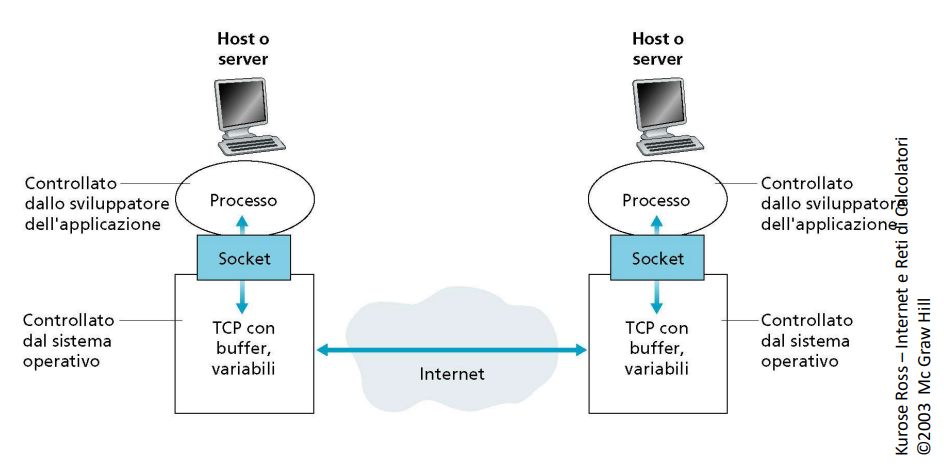
\includegraphics[scale=0.73]{identifprocesso.png}
I servizi di trasporto sono offerti al livello applicativo tramite le API. Ogni servizio di transport è \textbf{usato simultaneamente} da più processi application.\\
Come identifico i processi di livello application \textbf{di host diversi}? Serve un identificativo che identifichi sia l'host che il processo.\\
$\rightarrow$ Coppie \texttt{<Indirizzo IP, Numero di porta>}
\begin{center}
\fbox{
        \fbox{\parbox{6cm}{Indirizzo IP [32bit]}}
		\fbox{\parbox{4cm}{Numero di porta [16 bit]}}
}
\end{center}
\subsection{Esempio di API: TCP}
\begin{lstlisting}
Connection TCPopen(IPAddress, int)	//per aprire una connessione
void TCPsend(Connection, Data)		//per spedire dati su una connessione
Data TCPreceive(Connection)		//per ricevere dati da una connessione
void TCPclose(Connection)		//per chiudere una connessione
int TCPbind(int)			//per richiedere l'assegnazione della porta su
					//cui attendere le richieste di connessione

void TCPunbind(int)			//per liberare la porta assegnata
Connection TCPaccept(int)		//per attendere le richieste di connessione

//Connection: identificata da una quadrupla
//Astraggo dalle possibili eccezioni sollevate e dal loro trattamento
\end{lstlisting}
\pagebreak
\subsection{Uso dei Servizi di Trasporto}
Una coppia di processi fornisce servizi agli utenti di Internet, siano questi persone o applicazioni. La coppia di processi, tuttavia, \textbf{deve utilizzare i servizi offerti dal livello di trasporto} per la comunicazione, poiché non vi è una comunicazione fisica a livello applicativo. Le applicazioni di retesono quindi \textbf{realizzate \textit{sopra} ai servizi di trasporto dati}.\\
Nel livello trasporto dello stack protocollare TCP/IP sono previsti \textbf{due protocolli di trasporto principali}:
\begin{list}{}{}
\item \textbf{TCP} Transfer Control Protocol
\begin{list}{}{}
\item \textbf{Connection-Oriented}: è richiesto un setup tra client e server
\item Trasporto \textbf{affidabile} tra mittente e destinatario
\item \textbf{Controllo del flusso}: il mittente non \textit{inonderà} di dati il destinatario
\item \textbf{Controllo di congestione}: \textit{limita} il mittente quando la rete è satura
\item Non offre garanzie di timing né di ampiezza minima di banda
\end{list}
\item \textbf{UDP} User Datagram Protocol
\begin{list}{}{}
\item \textbf{Connectionless}
\item Trasporto \textbf{non affidabile}
\item \textbf{NO} controllo del flusso
\item \textbf{NO} controllo di congestione
\item \textbf{NO} garanzie di timing o di ampiezza minima di banda
\item \textit{Quindi quali applicazioni usano UDP, e perché?}
\end{list}
\end{list}
\paragraph{Che tipo di trasporto richiede un'applicazione?}
\subparagraph{Throughput} Anche detta \textbf{banda}, è la frequenza alla quale il processo mittente può inviare i bit al processo ricevente. Alcune applicazioni (es. multimedia) richiedono una \textbf{banda minima} per essere efficaci, altri (\textbf{elastic apps}) usano la banda che trovano a disposizione.\\Velocità di trasferimento $\neq$ velocità di propagazione
\subparagraph{Perdita di dati} Alcune applicazioni (es. audio) possono tollerare alcune perdite, altre (es. telnet, trasferimento file) richiedono un trasferimenti dati \textbf{affidabile} al 100%
\subparagraph{Timing} Alcune applicazioni (es. teleconferenze, videogame) richiedono un basso ritardo per essere efficaci
\begin{center}
\begin{tabbing}
\begin{tabular}{c | c c c }
\textbf{Applicazione} & \textbf{Tolleranza alla perdita dati} & \textbf{Throughput} & \textbf{Sensibilità al tempo}\\\hline\\
Trasferimento file & No & Variabile & No\\\\
Posta Elettronica & No & Variabile & No\\\\
Documenti Web & No & Variabile & No\\\\
Audio/Video in tempo reale & Si & \begin{tabular}{@{}c@{}}Audio: 5Kbps -- 1 Mbps\\Video: 10Kbps -- 5MKbps\end{tabular} & Si, centinaia di millisecondi\\\\
Audio/Video memorizzati & Si & \begin{tabular}{@{}c@{}}Audio: 5Kbps -- 1 Mbps\\Video: 10Kbps -- 5MKbps\end{tabular} & Si, pochi secondi\\\\
Videogame & Si & Fino a pochi Kbps & Si, centinaia di millisecondi\\\\
Messaggistica istantanea & No & Variabile & Si e no
\end{tabular}
\end{tabbing}
\end{center}
\pagebreak

\begin{center}
\begin{tabbing}
\begin{tabular}{c | c c }
\textbf{Applicazione} & \textbf{Protocollo a Livello Applicativo} & \textbf{Protocollo di Trasporto}\\\hline\\
Posta Elettronica & SMTP (RFC 2821) & TCP\\
Accesso a terminali remoti & Telnet (RFC 854) & TCP\\
Web & HTTP (RFC 2616) & TCP\\
Trasferimento file & FTP (RFC 959) & TCP\\
Streaming multimediale & HTTP (es. YouTube), RTP (RFC 1889) & TCP o UDP\\
Telefonia internet & SIP, RTP, proprietario (es. Skype) & Tipicamente UDP
\end{tabular}
\end{tabbing}
\end{center}
\section{Applicazioni Web e HTTP}
\subsection{Terminologia}
\paragraph{WEB} Consiste di \textit{oggetti} indirizzati da un \textbf{URL} (Uniform Resource Locator)
\paragraph{Pagine Web} Solitamente formate da: \textit{pagine WEB} (HTML, Javascript\ldots) e diversi \textbf{oggetti referenziati} (altre pagine, immagini, script\ldots)
\paragraph{Browser} Lo user agent per il web, ad esempio: Chrome, Firefox, Netscape, Lynx
\paragraph{Web server} Il server per il web, ad esempio: Apache, MS Internet Information Server
\subsection{Uniform Resource Identifier}
Una \textbf{URI} è una \textbf{forma generale per identificare una risorsa presente sulla rete} (IETF RFC 2396: \textit{una Uniform Resource Identifier è una stringa compatta di caratteri usata per identificare una risorsa astratta o fisica}).\\
La sintassi di uno URI è stata progettata ponendo la \textbf{trascrivibilità globale} come uno degli obiettivi principali: utilizza caratteri da un \textbf{alfabeto molto limitato} (es. le lettere dell'alfabeto latino base, numeri e qualche carattere speciale).\\
Uno URI può essere \textbf{rappresentato in molti modi}, ad esempio: inchiostro su carta, pixel su schermo, sequenza di ottetti\ldots L'\textbf{interpretazione di uno URI dipende soltanto dai caratteri utilizzati e non da come essi vengono rappresentati} nel protocollo di rete.
\subparagraph{Uniform} \textbf{Uniformità della sintassi} dell'identificatore, anche se i meccanismi per accedere alle risorse possono variare.
\subparagraph{Resource} Qualsiasi cosa abbia un'identità: documento, servizio, immagine, collezione di risorse\ldots
\subparagraph{Identifier} Oggetto che può agire da riferimento verso qualcosa che ha identità
\paragraph{}Esistono due tipi di URI:
\begin{list}{}{}
\item \textbf{URL} Uniform Resource Locator: sottotipo di URI che identifica una risorsa attraverso il suo \textbf{meccanismo di accesso primario}, ad esempio la \textit{posizione} nella rete.\\
\begin{list}{URL}{Esempi:}
\item \texttt{https://doi.org/10.1109/LCN.1988.10239}
\item \texttt{ftp://ftp.is.co.za/rfc/rfc1808.txt}
\item \texttt{https://www.apple.com/index.html}
\end{list}
\item \textbf{URN} Uniform Resource Name: sottotipo di URI che devono essere \textbf{globalmente univoci e persistenti}, anche quando la risorse cessa di esistere o di essere disponibile.\\
\begin{list}{URN}{Esempi:}
\item \texttt{urn:oasis:names:specification:docbook:dtd:xml:4.1.2:}
\item \texttt{urn:doi:10.1109/LCN.1988.10239}
\end{list}
\end{list}
\pagebreak
\subsubsection{Sintassi}
La sintassi di un URI è \textbf{organizzata gerarchicamente}, con le componenti \textbf{elencate in ordine decrescente} di importanza da sinistra a destra.\\
Una \textbf{URI assoluta} può essere formata da \textbf{quattro} componenti\\
\begin{center}
\texttt{<scheme>://<authority><path>?<query>}
\end{center}
\begin{list}{}{}
\item \texttt{<scheme>} \textbf{Obbligatorio}, schema per identificare la risorsa.\\
Lo URI scheme \textbf{definisce il namespace} dello URI, quindi potrebbe porre ulteriori vincoli su sintassi e semantica degli identificatori che usano quello schema. Nonostante molti URL scheme prendono il nome da protocolli, \textbf{questo non implica che l'unico modo di accedere} la risorsa dello URL \textbf{sia attraverso il protocollo specificato}.
\item \texttt{<authority>} Elemento gerarchico per richiamare un'authority così che la gestione del namespace definito sia delegato a quella authority. Il \textbf{nome di dominio} di un host o il suo \textbf{indirizzo IP} in notazione puntata decimale.\\
\texttt{authority = [userinfo@]host[:port]}
\item \texttt{<path>} Contiene dati specifici per l’authority (o lo scheme) e \textbf{identifica la risorsa nel contesto} di quello schema e di quella autorità. Può consistere in una sequenza di segmenti.
\item \texttt{<query>} L'interrogazione o i dati da passare alla risorsa richiesta
\end{list}
\begin{list}{}{Esempi:}
\item \texttt{foo://example.com:8042/over/there?name=ferret\#nose}
\begin{list}{}{}
\item \texttt{scheme = foo}
\item \texttt{authority = example.com:8042}
\item \texttt{path = /over/there}
\item \texttt{query = name=ferret}
\item \texttt{fragment = nose}
\end{list}
\item \texttt{urn:example:animal:ferret:nose}
\begin{list}{}{}
\item \texttt{scheme = urn}
\item \texttt{path = example:animal:ferret:nose}
\end{list}
\item \texttt{http://maps.google.it/maps/place?q=largo+bruno+pontecorvo+pisa\&hl=it}
\begin{list}{}{}
\item \texttt{scheme = http}
\item \texttt{authority = maps.google.it}
\item \texttt{path = /maps/place}
\item \texttt{query = q=largo+bruno+pontecorvo+pisa\&hl=it}
\end{list}
\end{list}
\subsubsection{Assolute e Relative}
Le URI possono essere assolute o relative.
\subparagraph{URI Assoluta} Identifica una risorsa \textbf{indipendentemente dal contesto} in cui è usata.
\subparagraph{URI Relativa} Informazioni per \textbf{identificare una risorsa in relazione ad un'altra URL} (è priva di \texttt{scheme} e \texttt{authority}). \textbf{Non viaggiano sulla rete}, sono interpretate dal browser in relazione al documento di partenza.
\pagebreak
\paragraph{Esempio di URI relativa}
Sia \texttt{http://a/b/c/d;p?q} il documento di partenza, allora
\begin{list}{}{}
\item \texttt{g} = \texttt{http://a/b/c/g}
\item \texttt{/g} = \texttt{http://a/g}
\item \texttt{//g} = \texttt{http://g}
\item \texttt{?y} = \texttt{http://a/b/c/?y}
\item \texttt{\#s} = \textit{documento corrente}\texttt{\#s}
\item \texttt{g;x?y\#s} = \texttt{http://a/b/c/g;x?y\#s}
\item \texttt{..} = \texttt{http://a/b/}
\item \texttt{../../g} = \texttt{http://a/g}
\end{list}
\section{HTTP}
Lo HTTP è usato dal 1990 come \textbf{protocollo di trasferimento per il World Wide Web}. Definito nel seguente modo (RFC 2068, RFC 2616): \textit{\textbf{procollo di livello applicazione} per sistemi di informazione distribuiti, collaborativi ed impermediali}.\\
Protocollo \textbf{generico}, \textbf{stateless} e \textbf{object-oriented} che può essere usato per molte attività, come name server e sistemi distribuiti di gestione oggetti, attraverso l'estensione dei suoi \textbf{request methods} (comandi). Una funzionalità dell'HTTP è la rappresentazione del tipo di dati, consentendo al sistema di essere \textbf{costruito indipendentemente dai dati che vengono trasferiti}.
\subsection{HTTP URL}
Lo schema \texttt{http} è usato per accedere alla risorsa attraverso il protocollo HTTP.
\paragraph{Sintassi} La sintassi per un URL http è:\\
\begin{center}
\texttt{http\_URL = http://host[:port][path]}
\end{center}
\begin{list}{}{}
\item \textbf{Host}: un dominio, hostname o indirizzo IP in forma decimale puntata di Internet.
\item \textbf{Porta}: un numero, se omessa viene usata la porta 80.
\end{list}
La risorsa è localizzata nel server in ascolto per connessioni TCP su quella porta di quell'host. Il path specifica la \textbf{Request-URI}.
\subsection{Caratteristiche}
Il protocollo HTTP è un protocollo \textbf{request/response}: la \textbf{connessione} viene \textbf{iniziata dal client}, che invia un \textbf{messaggio di request} al quale il server risponde con una \textbf{response}.\\
In quanto \textbf{generico e stateless} le coppie \textbf{richiesta/risposta sono indipendenti}.
\subsubsection{Modello} Il modello del protocollo HTTP è \textbf{client-server}:
\begin{list}{}{}
\item \textbf{Client}: browser che richiede, riceve e visualizza oggetti web.\\Stabilisce una connessione con il server e invia una \textbf{richiesta sotto forma di request-method, URI e versione di protocollo}, seguito da un messaggio.
\item \textbf{Server}: web server che invia oggetti in risposta ad una richiesta.\\Accetta le connessioni e serve le richieste rispondendo con i dati richiesti.
\end{list}
\subsubsection{Connessioni} Una \textbf{connessione} è un \textbf{circuito logico di livello trasporto} stabilito tra due programmi applicativi per comunicare tra loro.
\paragraph{Non-Persistent Connection} \texttt{http1.0: RFC 1945}\\Viene stabilita una \textbf{connessione TCP separata} per raggiungere ogni URL. \textbf{Aumenta il carico} sui server HTTP e \textbf{può causare congestioni su Internet} (questo perché, ad esempio, se vengono usate tante immagini allora si creano richieste multiple del solito server in un breve lasso di tempo).
\paragraph{Persistent Connection} \texttt{http1.1: RFC 2616}\\Se non è indicato altrimenti, il client può \textbf{assumere che il server manterrà una connessione persistente}.\\Lo standard specifica un \textbf{meccanismo con il quale} un client o un server \textbf{può segnalare la chiusura di una connessione TCP} (il campo \texttt{connection} nell'header). Una volta che la chiusura viene segnalata, il cliente \textbf{non deve più mandare richieste} su quella connessione.
\subsection{Esempio HTTP}
\texttt{Vedi slide}\footnote{https://elearning.di.unipi.it/pluginfile.php/27477/mod\_resource/content/2/L03\_Applicativo\_HTTP.pdf, slide 34}
\subsection{Messaggi HTTP}
\begin{center}
\texttt{generic-message = start-line *message-header CRLF [message-body]\\
start-line = Request-Line | Status-Line}
\end{center}
La \texttt{start-line} distingue \textbf{request} da \textbf{response}.\\\\
\textbf{HTTP Request Message}\\
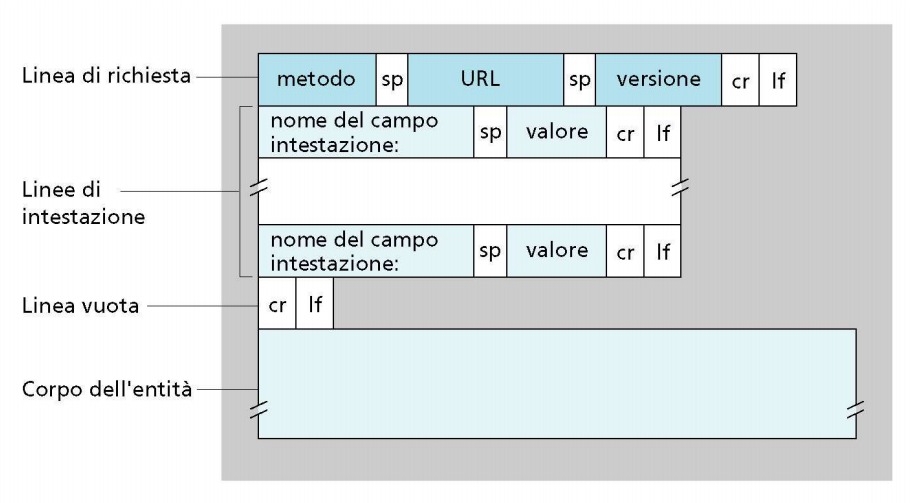
\includegraphics[scale=0.75]{httpmessage.png}\\
\textbf{HTTP Response Message}\\
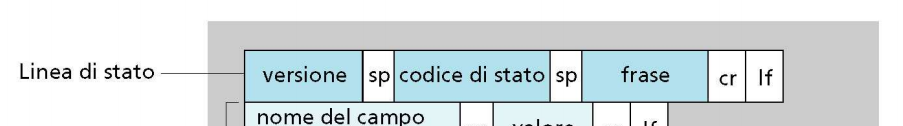
\includegraphics[scale=0.75]{httpresponse.png}
\pagebreak
\paragraph{HTTP Request} \texttt{Request-Line *( general-header | request-header | entity-header ) CRLF [message-body]}
Ad esempio:\\
\texttt{GET /pub/WWW/TheProject.html HTTP/1.1\\
Host: www.w3.org\\
Connection: close\\
User Agent: Mozilla/4.0\\
Accept-language: it\\\\
(Body)}
\subparagraph{HTTP Request Line} \texttt{Request-Line = Method SP Request-URI SP HTTP-Version CRLF}\\\texttt{GET http://www.w3.org/pub/WW/TheProject.html HTTP/1.1}
\begin{list}{}{}
\item \texttt{Method = GET}
\item \texttt{Request-URI = http://www.w3.org/pub/WW/TheProject.html}
\item \texttt{HTTP-Version = HTTP/1.1}
\end{list}
\texttt{Method = "OPTIONS" | "GET" | "HEAD" | "POST" | "PUT" | "DELETE" | "TRACE" | extension-method}\\
\begin{list}{}{}
\item \textbf{Method}: indica il \textbf{metodo che deve essere eseguito} sulla risorsa identificata dal \texttt{Request-URI}. \textbf{Case sensitive}.
\item \textbf{HTTP-Version}: indicare la versione del protocollo è pensato per consentire al mittente di indicare il formato di un messaggio e la sua capacità di capire il resto della comunicazione HTTP.
\item Le \textbf{URI} sono stringhe formattate in modo semplice che identificano una risorsa di rete.
\subsection{Header}
Gli \textbf{header} sono insiemi di coppie <nome:valore> che \textbf{specificano alcuni parametri} del messaggio trasmesso o ricevuto.
\begin{list}{}{}
\item \textbf{General header} Relativi alla trasmissione
\begin{list}{}{}
\item \textbf{Data}: data e ora di generazione del messaggio
\item \textbf{Connection}: consente al mittente di specificare le opzioni desiderate per quella particolare connessione. L'opzione "close" segnala che la connessione verrà chiusa al completamento della response
\item \textbf{Transfer-encoding}: indica quale (se presente) tipo di trasformazione è stata applicata al message body per trasferirlo correttamente dal mittente al destinatario (chunked, gzip\ldots)
\item \textbf{Cache Control}
\begin{list}{}{}
\item \textbf{Public} Indica che la response è cachable in qualsiasi cache
\item \textbf{Private} Indica che tutte o parti della response sono destinate ad un singolo utente e \textbf{non devono essere} memorizzate in una cache condivisa (shared cache). Una cache privata (non-shared) potrebbe memorizzare la response
\item \textbf{no-cache} Indica che tutte o parti della response \textbf{non devono essere memorizzate in nessuna cache}
\end{list}
\end{list}
\texttt{general-header = Cache-Control | Connection | Date | Pragma | Transfer-Encoding | Upgrade | Via}\\Questi header si applicano \textbf{a tutto il messaggio}. Esempi:
\begin{list}{}{}
\item \texttt{Date: Tue, 15 Nov 1994 08:12:31 GMT}
\item \texttt{Connection: close}
\item \texttt{Transfer-Encoding: chunked}
\end{list}
\item \textbf{Entity header} Relativi all'entità trasmessa\\Content-type, Content-length, data di scadenza\ldots
\item \subsubsection{Request header} Relativi alla richiesta\\Chi fa la richiesta, a chi viene fatta, che tipo di caratteristiche è in grado di accettare il client, autorizzazione\ldots consente al client di passare \textbf{informazioni aggiuntive} a proposito della richiesta o del client stesso al server. Questi campi agiscono come \textbf{modificatori di richiesta}, con \textbf{semantica equivalente a quella dei parametri} di un metodo.\\
\texttt{request-header = Accept | Accept-Charset | Accept-Encoding | Accept-Language | Authorization | Proxy-Authorization | From | Host | If-Modified-Since | If-Unmodified-Since | If-Match | If-None-Match | If-Range | Max-Forwards | Range | Referer | User-Agent}\\
\begin{list}{}{}
\item \textbf{Accept} Specifica che tipi di media sono accettabili nella response. Parametro \texttt{q} per indicare un fattore di qualità relativo, default a 1.
\item \textbf{Accept-Charset} Indica il set di caratteri accettato per la risposta
\item \textbf{Accept-Encoding} Tipi di trasformazioni accettate (es. compressione)
\item
\item \texttt{Accept: text/plain;q=0.5, text/html, text/x-dvi;q=0.8, text/x-c}
\item \texttt{Accept-Charset: iso-8859-5, unicode-1-1;q=0.8}
\item \texttt{Accept-Encoding: compress, gzip}
\end{list}
\begin{list}{}{(Alcuni) metodi request:}
\item \textbf{OPTIONS} Richiede \textbf{solo le opzioni di comunicazione} associate ad un URL o al server stesso (capacità, metodi esposti ecc.). Un esempio:\\
\texttt{OPTIONS http://192.168.11.66/manual/index.html HTTP/1.1\\host: 192.168.11.66\\
Connection: close\\\\
HTTP/1.1 200 OK\\
Date: Sun, 14 May 2000 19:52:12 GMT\\
Server: Apache/1.3.9 (Unix) (Red Hat/Linux)\\
Content-Length: 0\\
Allow: GET, HEAD, OPTIONS, TRACE\\
Connection: close\\}
\item \textbf{GET} Richiede il trasferimento di una risorsa identificata da un URL o le operazioni associate all'URL stessa. Un esempio:\\
\texttt{GET http://192.168.11.66 HTTP/1.1\\
host: 192.168.11.66\\
Connection: close}\\\\
Response\\
\texttt{HTTP/1.1 200 OK\\
Date: Sun, 14 May 2000 19:57:13 GMT\\
Server: Apache/1.3.9 (Unix) (Red Hat/Linux)\\
Last-Modified: Tue, 21 Sep 1999 14:46:36 GMT\\
ETag: "f2fc-799-37e79a4c"\\
Accept-Ranges: bytes\\
Content-Length: 1945\\
Connection: close\\
Content-Type: text/html\\\\
<!DOCTYPE HTML PUBLIC "-//W3C//DTD HTML 3.2\\
Final//EN">\\
<HTML>\ldots\\}
Sono possibili \textbf{GET condizionali e parziali}. Esempio di GET condizionale:\\
\texttt{GET http://192.168.11.66 HTTP/1.1\\
Host: 192.168.11.66\\
If-Modified-Since: Tue, 21 Sep 1999\\
14:46:36 GMT}\\\\
Response:\\
\texttt{HTTP/1.1 304 Not Modified\\
Date: Wed, 22 Sep 1999 15:06:36 GMT\\
Server: Apache/1.3.9 (Unix) (RedHat/Linux)}\\
\item \textbf{HEAD} Simile al GET, ma il server \textbf{non trasferisce il body} nella response. Utile per controllare lo stato dei documenti (validità, modifiche\ldots). Un esempio:\\
\texttt{HEAD http://192.168.11.66 HTTP/1.1\\
host: 192.168.11.66\\
Connection: close}\\\\
Response (notare la somiglianza con GET, esclusa la mancanza qua del body):\\
\texttt{HTTP/1.1 200 OK\\
Date: Sun, 14 May 2000 20:02:41 GMT\\
Server: Apache/1.3.9 (Unix) (Red Hat/Linux)\\
Last-Modified: Tue, 21 Sep 1999 14:46:36 GMT\\
ETag: "f2fc-799-37e79a4c"\\
Accept-Ranges: bytes\\
Content-Length: 1945\\
Connection: close\\
Content-Type: text/html}\\
\item \textbf{POST} Serve per \textbf{inviare dal client al server} informazioni inserite nel body del messaggio.\\In teoria lo standard dice che il metodo POST è usato per richiedere che il server \textbf{accetti l'entità racchiusa nella richiesta come nuovo suboordinato della risorsa identificata} dallo Request-URI nel Request-Line.\\\textbf{Nella pratica}, \textbf{la funzionalità effettiva del metodo POST} è \textbf{determinata dal server} e solitamente dipende dalla Request-URI.\\
\item \textbf{DELETE} Il client \textbf{chiede di cancellare una risorsa identificata} dalla Request-URI.\\Solitamente non attivo su server pubblici.\\
\item \textbf{PUT} Il client \textbf{chiede di creare/modificare una risorsa identificata} dalla Request-URI. Dopo posso usare una GET per recuperarla.\\Solitamente non attivo su server pubblici.
\end{list}
\item \textbf{Response header} Nel messaggio di risposta\\Server, autorizzazione richiesta\ldots
\end{list}
\paragraph{Safe Methods} Metodi che \textbf{non hanno effetti collaterali} (es. non modificano la risorsa): GET, HEAD, OPTIONS, TRACE
\paragraph{Idempotent Methods} Metodi che \textbf{non hanno effetti ulteriori se vengono fatti N > 0 richieste identiche}: GET, HEAD, PUT, DELETE, OPTIONS, TRACE
\end{list}
\pagebreak
\subsection{HTTP Response}
\begin{center}
\texttt{Response = Status-Line *( general-header | response-header | entity-header ) CRLF [message-body]}
\end{center}
Un esempio:\\
\texttt{HTTP/1.1 200 OK\\
Date: Sun, 14 May 2000 23:49:39 GMT\\
Server: Apache/1.3.9 (Unix) (Red Hat/Linux)\\
Last-Modified: Tue, 21 Sep 1999 14:46:36 GMT}\\
\paragraph{Status-Line} La prima linea del messaggio di risposta.\\
\texttt{Status-Line = HTTP-Version SP Status-Code SP Reason-Phrase CRLF}\\Esempio: \texttt{HTTP/1.1 200 OK}
\subparagraph{Status-Code} Intero a 3 cifre, risultato del tentativo di comprendere e soddisfare la richiesta.\\\begin{center}
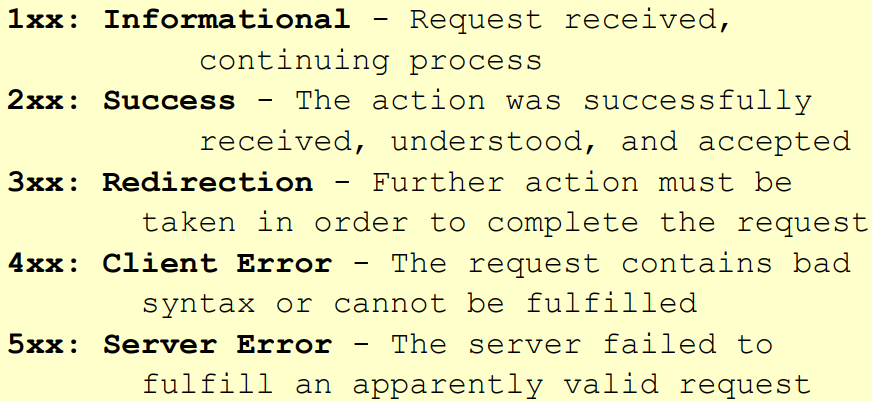
\includegraphics[scale=0.5]{httpresponsecode.png}\\\texttt{http://www.w3.org/Protocols/rfc2616/rfc2616-sec10.html}
\end{center}
\subparagraph{Reason-Phrase} Ha l'obiettivo di fornire una breve descrizione testuale dello Status-Code. Lo Status-Code è indirizzato ai computer mentre la Reason-Phrase è per gli umani.
\subsubsection{Response Headers} Il campo response-header consente al server di passare ulteriori informazioni sulla response. Questi campi dell'header forniscono informazioni sul server e sull'accesso alla risorsa identificata dallo Request-URI.\\
\texttt{response-header = Age | Location | Proxy-Authenticate | Public | Retry-After | Server | Vary | Warning | WWW-Authenticate}\\\\Esempio:\\
\texttt{Age: 150 // età del doc. se tramite Proxy\\
Location: http://www.w3.org/pub/WWW/People.html\\
Server: CERN/3.0 libwww/2.17}
\begin{list}{}{}
\item \textbf{Age} Una stima in secondi del tempo passato dalla generazione della risposta dal server di origine
\item \textbf{Location} Usato per reindirizzare il ricevente verso una destinazione diversa dalla Request-URI per il completamento della richiesta o l'identificazione di una nuova risorsa
\item \textbf{Server} Informazioni sul software usato dal server d'origine per gestire la richiesta
\end{list}
\subsection{Negoziazione del contenuto}
Le risorse possono essere \textbf{disponibili in multiple rappresentazioni}, ad esempio più lingue, formati, dimensioni e risoluzioni, o variare in altri modi ancora. La \textbf{content negotiation} è il meccanismo usato per \textbf{selezionare l'appropriata rappresentazione} quando si serve una richiesta. Ogni entità è costituita da un \textbf{entity body} e da una serie di \textbf{entity headers} che ne definiscono il contenuto e le proprietà. Gli entity header sono \textbf{informazioni sulle informazioni}, cioè \textbf{metadati}.
\subsubsection{Entity Headers}
\texttt{entity-header = Allow | Content-Base | Content-Encoding | Content-Language | Content-Length |\\Content-Location | Content-MD5 | Content-Range | Content-Type | ETag | Expires | Last-Modified |\\extension-header}
\begin{list}{}{}
\item \textbf{Content-Base} URI assoluta da usare per risolvere le URL relative contenute nell'entity-body
\item \textbf{Content-Encoding} Codifica dell'entity-body (es. gzip)
\item \textbf{Content-Language} Lingua dell'entity-body (es. en, it)
\item \textbf{Content-Type} Tipo dell'entity-body (es. text/html)
\item \textbf{Expires} Valore temporale dell'entity-body (utile nel caching)
\item \textbf{Last-Modified} Data dell'ultima modifica sul server (utile nel caching)
\end{list}
\section{Web Caching}
L'obiettivo è \textbf{soddisfare una richiesta} del cliente \textbf{senza contattare il server}. Si \textbf{memorizzano copie temporanee delle risorse web} (es. pagine HTML e immagini) e si servono al client per ridurre l'uso di risorse (es. banda e workload sul server), diminuendo anche il tempo di risposta.
\paragraph{User Agent Cache} lo \textbf{user agent} (il browser) mantiene una \textbf{copia delle risorse visitate dall'utente}.
\paragraph{Proxy Cache} Il proxy intercetta il traffico e \textbf{mette in cache le risposte}. Le successive richieste alla stessa Request-URI \textbf{possono essere servite dal proxy senza inoltrare la richiesta} al server.
\subparagraph{Proxy} Programma intermediario che agisce sia da server che da client, con l'obiettivo di fare richieste per conto di altri client. Le richieste sono servite internamente o passandole oltre, anche traducendole, ad altri server.
\section{Cookies}
L'HTTP è \textbf{stateless}, per cui non mantiene info sui client. Come posso riconoscere il cliente di un'applicazione web (es. Amazon)? Come posso realizzare applicazioni web con stato (es. carrello della spesa)? Ricordiamo che \textbf{tipicamente l'utente si connette ogni volta con un indirizzo IP e porta diversi}.\\
\textbf{Soluzione}: \textbf{numerare i client} e obbligarli a \textbf{farsi riconoscere ogni volta presentando un cookie}.
\paragraph{Funzionamento} Il client C invia al server S una normale richiesta HTTP.\\
Il server invia la normale risposta + una linea \textbf{Set-Cookie: 1678453}\\
Il client memorizza il cookie in un file associato a S, e aggiunge una linea \textbf{Cookie: 1678453} a \textbf{tutte le successive richieste} verso quel sito.\\
Il server confronta il cookie presentato con l'informazione che ha associato a quel cookie.
\paragraph{Utilizzi} I cookie vengono utilizzati per:
\begin{list}{-}{}
\item Autenticazione
\item Ricordare il profilo utente e le scelte precedenti (alla carta-socio)
\item Creare sessioni sopra un protocollo stateless (es. carrelli della spesa)
\end{list}
\textbf{Non accettare dolci dagli sconosciuti}: \texttt{cookiecentral.com}
\pagebreak
% https://elearning.di.unipi.it/pluginfile.php/27733/mod_resource/content/1/L04_Applicativo_FTP_telnet.pdf
\section{Telnet}
\paragraph{TErminaL NETwork} Protocollo di terminale remoto che permette l'\textbf{uso interattivo} di macchine remote: \textbf{accesso remoto}, \textbf{accessu multiplo ad un singolo computer}.\\
Realizza coppie client-server generiche per login remoto, non specializzate per tipo di applicativo. Invece di offrire server specializzati per servizi interattivi, l'approccio consiste nel permettere all'utente di \textbf{effettuare una sesisone login nella macchina remota} e quindi \textbf{inviare i comandi}. Tramite il login remoto gli utenti hanno accesso ai comandi e ai programmi disponibili nella macchina remota.

\textit{Puoi mandare comandi attraverso il programma Telnet e verranno eseguiti come se fossi a scriverli direttamente sulla server console. Questo ti consente di controllare il server e comunicare con gli altri server sulla rete}\\
\textbf{Non è un compito facile}, per realizzarlo il Telnet:
\begin{list}{}{}
\item \textbf{Maschera} sia la rete che i S.O.
\item Utilizza un'\textbf{interfaccia minima ma veloce}, tipicamente a caratteri
\end{list}
\subsection{Introduzione}
Telnet permette ad un utente su una macchina di \textbf{stabilire una connessione con un login su server remoto}.\\In seguito, passa la \textbf{battute dei tasti} della macchina locale \textbf{alla macchina remota}: i comandi vengno \textbf{eseguiti come se fossero stati battuti al terminale della macchina remota}.\\Dopodiché, l'\textbf{output} della macchina remota \textbf{viene trasportato al terminale utente}.\\\\
Questo è un \textbf{servizio trasparente}: il terminale dell'utente \textit{sembra} essere \textbf{connesso direttamente} alla macchina remota\\\\
\begin{list}{}{Il modello di Telnet include:}
\item \textbf{Server} che \textbf{accetta} le richieste
\item \textbf{Client} che \textbf{effettua} le richieste
\item \textbf{Il programma Telnet} che svolge due funzioni:
\begin{list}{}{}
\item \textbf{Interagisce col terminale utente} sull'host locale
\item \textbf{Scambia messaggi} con il Telnet server
\end{list}
\end{list}
\subsection{Protocollo Telnet}
\paragraph{RFC 854} Comunicazione generale, bidirezionale e orientata a blocchi di 8bit. L'obiettivo primario è di fornire un metodo standard per \textbf{interfacciare dispositivi terminali e processi terminal-oriented tra loro}.\\
Usa il TCP, con una connessione TCP persistente per tutta la durata della sessione di login, sulla porta 23 del server.
\begin{list}{}{}
\item Client \textbf{stabilisce una connessione TCP} con il server
\item Client \textbf{accetta le battute di tasti} sul terminale \textbf{e le invia al server}.\\
\textbf{Accetta i caratteri} che il server manda indietro \textbf{e li visualizza} sul terminale utente.
\item Server \textbf{accetta la connessione TCP} e trasmette i dati al S.O. locale.\\\\
\end{list}
\begin{multicols}{2}
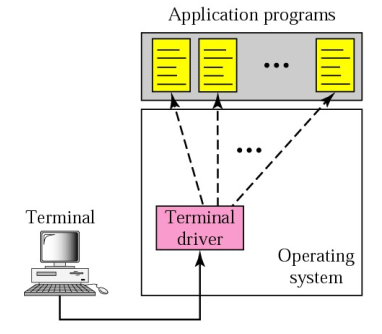
\includegraphics[scale=0.5]{locallogin.png}\\
In \textbf{Local Login} il S.O. assume che gli input ad un processo vengano forniti dallo standard input (tastiera) e che gli output siano inviati allo standard output (monitor).
\end{multicols}
\pagebreak
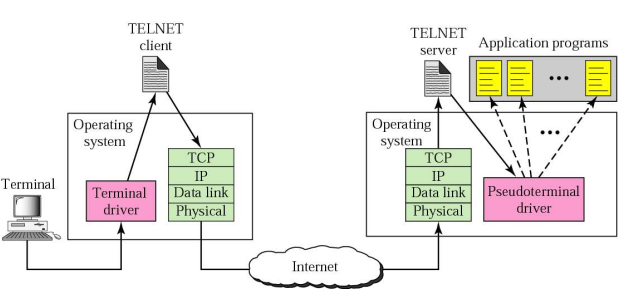
\includegraphics[scale=0.75]{remotelogin.png}\\
In \textbf{Remote Login} lo \textbf{Pseudo Terminal Driver} è l'entry point del S.O. che consente di trasferire caratteri ad un processo \textbf{come se provenissero dal terminale}. Ha il compito di \textbf{accettare i caratteri} dal server e \textbf{trasmetteri al S.O} che li consegnerà all'applicazione opportuna.
\subsection{NVT}
Il Telnet deve \textbf{poter operare con il numero massimo di sistem}, quindi gestire \textbf{dettagli di S.O. eterogenei} che possono differire per:
\begin{list}{}{}
\item \textbf{Set di codifica} dei caratteri
\item \textbf{Lunghezza} della linea e della pagina
\item \textbf{Tasti funzione} individuati da diverse sequenze di caratteri (\textbf{escape sequence})\\
Es. diverse combinazioni per interrompere un processo(\texttt{CTR+C}, \texttt{ESC}), caratteri ASCII diversi per la terminazione di righe di testo.
\end{list}
Per risolvere questo problema si definisce \textbf{un ambiente virtuale}. Sulla rete si considera un \textbf{unico terminale standard} e in corrispondenza di ogni stazione di lavoro si effettuano le \textbf{conversioni da terminale locale a terminale virtuale e viceversa}.
\paragraph{Network Virtual Terminal} Telnet assume che sui due host sia in esecuzione un \textbf{Network Virtual Terminal}, la connessione TCP è stabilita tra i due terminali NVT.\\
L'NVT è un dispositivo \textit{immaginario} che \textbf{fornisce una rappresentazione astratta di un terminale canonico}. Gli host, sia client che server, traducono le loro caratteristiche locali così da \textbf{apparire esternamente come un NVT} e assumo che l'host remoto sia un NVT.\\\\
Il Network Virtual Terminal definisce un \textbf{set di caratteri e di comandi} universale, che permette di:
\begin{list}{}{}
\item \textbf{Trasformare il set di caratteri in uso} localmente \textbf{in un set di caratteri universale} (lettere accentate, tasti freccia, backspace\ldots), includendo anche i caratteri di controllo più importanti (break\ldots)
\item \textbf{Inviare i caratteri di controllo in maniera privilegiata} (meccanismo URGENT del TCP)
\end{list}
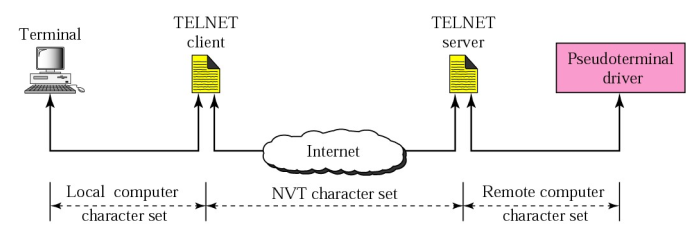
\includegraphics[scale=0.75]{NVT.png}\\
\subsection{Architettura}
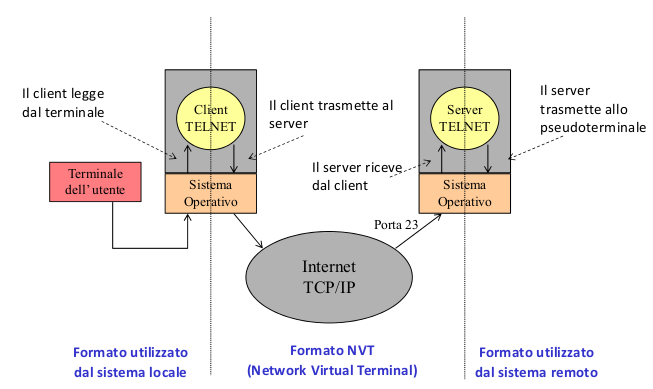
\includegraphics[scale=0.75]{telnetarch.png}
\pagebreak
\subsection{Funzionamento}
Rispetto alla esecuzione in locale, sono aggiunti una \textbf{serie di intermediari}:
\begin{list}{}{}
\item Il client Telnet \textbf{trasforma in NVT} ed usa il S.O. per inviare sulla rete;
\item la rete ed il S.O. server portano i dati al server Telnet;
\item il server Telnet \textbf{traduce da NVT a S.O.} remoto;
\item il S.O. remoto \textbf{esegue} il dovuto;
\item si percorre il cammino inverso con gli stessi soggetti.
\end{list}
Un esempio:
\begin{enumerate}
\item L'utente digita \texttt{INVIO} sulla tastiera
\item Il S.O. passa al client il carattere \texttt{CR}
\item Il client converte \texttt{CR} in \texttt{CR-LF} e lo invia sulla connessione TCP
\item Il server riceve \texttt{CR-LF}, lo converte in \texttt{LF} e lo passa allo pseudoterminale
\item Lo pseudoterminale passa all'applicazione \texttt{LF}
\item L'applicazione esegue l'operazione di \texttt{INVIO}
\end{enumerate}
\paragraph{Formato} I terminali NVT si scambiano i dati in \textbf{formato 7bit US-ASCII}. Ogni carattere è inviato come un ottetto con il primo bit settato a 0. I byte con il bit più significativo a 1 sono usati per le \textbf{sequenze di comandi}.\\
I comandi (es. end-of-line trasmesso come la seuqenza \texttt{CR-LF}) iniziano con un ottetto speciale (\textbf{Interpret as Command} o \texttt{IAC}) di 1 $\rightarrow$ \textbf{Inband Signalling} (comandi e dati sulla stessa connessione).\\\\
I messaggi di controllo iniziali sono usati per scambiare informazioni sulle caratteristiche degli host (\textbf{Telnet  Option Negotiation}).\\
\paragraph{Comandi} Qualche esempio
\begin{center}
\begin{tabular}{c | c c}
\textbf{Comando} & \textbf{Codifica Decimale} & \textbf{Significato} \\
\texttt{IAC} & 255 & Interpreta come comando l'ottetto successivo \\
\texttt{EL} & 248 & Erase Line \\
\texttt{EC} & 247 & Erase Character \\
\texttt{IP} & 244 & Interrupt Process \\
\texttt{EOR} & 239 & End of Record \\
\end{tabular}
\end{center}
\paragraph{NVT conviene?} Suppongo di voler far interoperare N sistemi.\\
Senza usare NVT, ho bisogno di scrivere N-1 client per ogni sistema, e N server (uno per sistema) = \textbf{devo scrivere N(N-1)+N applicazioni}.\\
Usando NVT invece devo scrivere soltanto N server e N client, cioè \textbf{2N applicativi}.\\
Per N $>$ 2 conviene NVT.
\pagebreak
\section{SSH}
Poiché Telnet passa tutto in chiaro, \textbf{anche le password}, con il tempo si è resa necessaria una maggiore sicurezza.
\paragraph{Secure Shell} SSH è un'applicazione nata per \textbf{sostituire Telnet} e \textbf{risolvere i suoi problemi di sicurezza}. Facilita la comunicazione sicura tra client e server e permette la login remota, resa sicura attraverso \textbf{tecniche di cifratura}. Nella realtà SSH offre \textbf{funzionalità molto superiori} a quelle di Telnet\footnote{Vedi su Forouzan}.
\begin{multicols}{2}
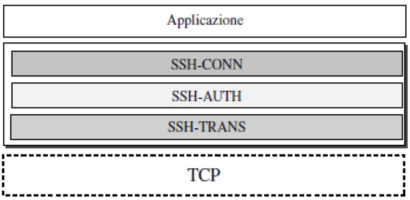
\includegraphics[scale=0.55]{stackssh.png}\\
\columnbreak

\paragraph{SSH-TRANSPORT} Realizza la \textbf{connessione sicura} tra due host:
\begin{list}{}{}
\item Autenticazione del server
\item Negoziazione degli algoritmi di cifratura
\item Scambio di chiavi
\end{list}
\paragraph{SSH-AUTHENTICATION} Meccanismi per autenticare l'utente
\paragraph{SSH-CONNECTION} Sessioen di login remoto, tunneling
\end{multicols}
\section{TCP Port Forwarding}
\paragraph{Port Forwarding} L'inoltro delle porte è un meccanismo che permette di creare un \textbf{canale di comunicazione sicuro} attraverso il quale veicolare qualsiasi tipo di connessione TCP.\\
Viene \textbf{creato un canale di comunicazione cifrato tra la porta all'indirizzo remoto} al quale ci si vuole collegare \textbf{ed una porta locale libera}. In questo modo le applicazioni punteranno il collegamento alla porta locale e la connessione verrà \textbf{inoltrata automaticamente} all'host remoto tramite un canale sicuro.\\
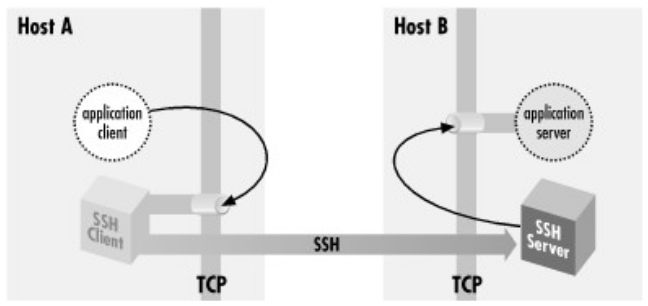
\includegraphics[scale=0.75]{portforwarding.png}\\\\
\texttt{ssh -L 123:localhost:456 remotehost}

\texttt{-L} specifica che la data porta sull'host locale è da 

inoltrare alal data porta sull'host remoto.\\

\texttt{<porta locale>:<host>:<porta remota di host>}
\pagebreak
\section{FTP}
Il \textbf{File Transfer Protocol} (\texttt{RFC 959}) è usato per il \textbf{trasferimento di file da/a un host remoto}. Segue il modello client server:
\begin{list}{}{}
\item Client: il lato che \textbf{chiede} il trasferimento
\item Server: l'host remoto
\end{list}
\paragraph{Standard} Nelle reti TCP/IP lo FTP è lo \textbf{standard per il trasferimento di file}. Questo è un servizio \textbf{diverso} dall'accesso condiviso online (che è un \textbf{accesso simultaneo} da parte di più programmi \textbf{ad un singolo file}).\\
\begin{list}{}{L'FTP fornisce anche \textbf{funzionalità aggiuntive} oltre al semplice trasferimento di file:}
\item \textbf{Accesso interattivo}: l'utente può \textbf{navigare} e \textbf{cambiare/modificare} l'albero di directory nel file system remoto
\item \textbf{Specifica del formato} dei dati da trasferire (es. file di testo o file binari)
\item \textbf{Autenticazione}: il client può specificare username e password
\end{list}
\subsection{Modello FTP}
\begin{list}{}{L'FTP ha \textbf{due tipi di connessione}:}
\item \textbf{Control connection}: scambio di comandi e risposte tra client e server, segue il protocollo Telnet
\item \textbf{Data connection}: connessione su cui i dati sono trasferiti con modi e tipi specificati. I dati trasferiti possono essere \textbf{parte} di file, \textbf{un} file o \textbf{un set} di file.
\end{list}
\subsubsection{Connessione di Controllo}
Il client FTP \textbf{contatta il server FTP alla porta 21} usando il TCP come protocollo di trasporto. Il client \textbf{ottiene l'autorizzazione} sulla connessione di controllo (es. cambio directory, invio file ecc\ldots).\\
La \textbf{connessione} è \textbf{persistente}.
\subsubsection{Connessione Dati}
Quando il server riceve un comando per trasferire file (da o verso il client), \textbf{apre una connessione TCP} con il client.\\ \textbf{Active Mode}: una connessione per ciascun trasferimento e dopo il trasferimento di un file il server chiude la connessione.\\\\
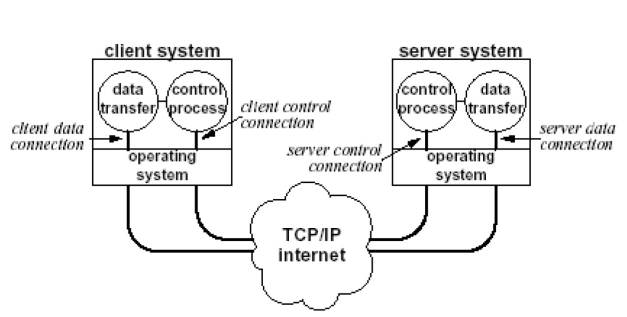
\includegraphics[scale=0.75]{modelloftp.png}
\pagebreak
\subsection{Altri Dettagli}
\begin{list}{}{}
\item Quando un client attiva la connessione di controllo con il server usa un \textbf{numero di porta assegnato localmente in modo casuale} e contatta il server ad una porta nota, cioè la 21
\item FTP usa la connessione di controllo per permettere a client e server di \textbf{coordinare l'uso delle porte assegnate dinamicamente} per il trasferimento dati
\item La \textbf{connessione di controllo} FTP \textbf{si basa sul protocollo Telnet}
\item \subsubsection{Due Modalità} Per creare la connessione TCP per il trasferimento dati sono possibili due modalità:
\begin{list}{}{}
\item \textbf{Active Mode}: vedi sopra, una connessione per ciascun trasferimento e dopo il trasferimento di un file il server chiude la connessione. Il server deve conoscere il numero di porta lato client (glielo comunica)
\item \textbf{Passive Mode}: il \textbf{client ottiene un numero di porta dal server} (porta 20, non necessariamente).\\
Il server non deve accettare connessioni da un processo arbitrario.\\\
Da \texttt{RFC 959} -- PASV: questo comando richede che il server-DTP "ascolti" su una porta dati (che non è quella predefinita) e di aspettare una connessione piuttosto che iniziarne una alla ricezione del comando di trasferimento. La risposta a questo comando include l'host e l'indirizzo e porta su cui il server sta ascoltando.
\end{list}
\end{list}
\textbf{DTP}: Data Transfer Process\\
\textbf{PI}: Protocol Interpreter\\
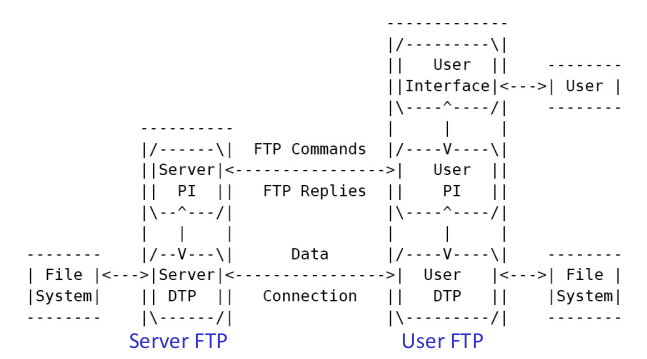
\includegraphics[scale=0.75]{modelloftp2.png}
\begin{list}{}{}
\item \textbf{I dispositivi} dove risiedono client e server FTP \textbf{sono diversi}: S.O., diverse strutture per gestire i file, diversi formati dei file\ldots
\item Per effettuare il trasferimento di file, il client deve \textbf{definire il tipo di file}, la \textbf{struttura dati} e la \textbf{modalità di trasmissione} al fine di risolvere i problemi di eterogeneità tra client e server.
\item Il \textbf{trasferimento file} viene \textbf{preparato attraverso uno scambio di informazioni lungo la connessione di controllo}
\item La \textbf{comunicazione} sulla connessione di controllo \textbf{avviene per mezzo di caratteri con una codifica standard NVT ASCII}, sia per i comandi che per le risposte
\item \subsubsection{Stateful} \textbf{FTP è un protocollo stateful}. Il server deve \textbf{tenere traccia dello stato} dell'utente: tra le altre cose anche della connessione di controllo associata ad un account e della directory attuale.
\item \subsubsection{Modalità di trasmissione}
\begin{list}{}{}
\item \textbf{Stream mode}: FTP invia i dati a TCP con un \textbf{flusso continuo di bit}
\item \textbf{Block mode}: FTP invia i dati a TCP \textbf{suddivisi in blocchi}, ognuno dei quali \textbf{preceduto da un header}
\item \textbf{Compressed mode}: si trasmette il \textbf{file compresso}
\end{list}
\end{list}
\subsection*{Comandi di Controllo}
\begin{list}{}{}
\item \texttt{USER username}
\item \texttt{PASS password}
\item \texttt{LIST}, elenca i file della directory corrente
\item \texttt{NLST}, richiede l'elenco di file e directory (\texttt{ls})
\item \texttt{RETR filename}, recupera (\texttt{get}) un file dalla directory corrente
\item \texttt{STOR filename}, memorizza (\texttt{put}) un file nell'host remoto
\item \texttt{ABOR}, interrompe l'ultimo comando ed i trasferimenti in corso
\item \texttt{PORT}, indirizzo e numero di porta del client
\item \texttt{SYST}, il server restituisce il tipo di sistema
\item \texttt{QUIT}, chiude la connessione
\end{list}
\subsection*{Codici di Ritorno}
I codici di ritorno sono composti da un codice di stato e da un'espressione, come in HTTP:
\begin{list}{}{}
\item \texttt{331 Username OK, password required}
\item \texttt{425 Can't open data connection}
\item \texttt{452 Error writing file}
\item \texttt{200 Comando OK}
\item \texttt{125 Data connection already open, transfer starting}
\item \texttt{225 Data connection open}
\item \texttt{225 Closing data connection. Requested file action succesful} (es. trasferimento file o \texttt{ABOR})
\item \texttt{426 Connection closed, transfer aborted}
\item \texttt{227 Entering passive mode}
\end{list}
\subsection{Anonymous FTP} Server che supportano connessioni FTP senza autenticazione, spesso consentendo operazioni limitate.\\
\texttt{ftp.ed.ac.uk}, user: \texttt{ftp} e password la mail.
\pagebreak
\section{DNS}
\paragraph{Identificare il processo} Ogni processo di livello applicativo ha necessità di \textbf{individuare il processo omologo} con il quale vuole comunicare. Il processo omologo \textbf{risiede su una} particolare \textbf{macchina remota anch'essa da indivudare} (sappiamo che usa lo stesso protocollo).
\subparagraph{Nome} Uno \textbf{nome identifica un oggetto}. Consiste in una sequenza di caratteri scelti da un alfabeto finito, scelta per scopo mnemonico.\\
Nome significativo di alto livello (alfanumerico), vero e proprio identificativo di livello applicativo.
\subparagraph{Indirizzo} Un \textbf{indirizzo identifica dove tale oggetto è situato}.\\
Host di internet usano indirizzi IP (32bit) per instradare i datagrammi (livello di rete). Il formato è scelto per garantire l'efficienza dell'instradamento.\\
\textbf{Disaccoppiamento}: ad un nome possono essere associati più indirizzi.\\\\
\textbf{Come associare indirizzo IP e nome?}
\subsection{Motivazioni}
\paragraph{Inizi} All'inizio l'associazione fra nomi logici e indirizzi IP era \textbf{statica}: tutti i nomi logici ed i relativi indirizzi erano contenuti in un file (\textbf{host file}) periodicamente aggiornato da un server ufficiale. Questo approccio è infattibile nella rete internet attuale:
\begin{list}{}{}
\item Non è possibile che \textbf{ogni host mantenga una copia aggiornata} dell'elenco. Questo per dimensioni dell'elenco, per i volumi di traffico per trasferire i cambiamenti\ldots
\item Non è possibile \textbf{centralizzare un elenco del genere}: si avrebbe così un unico punto di fallimento, un gigantesco volume di traffico sul server\ldots\\
Questa soluzione non è scalabile.
\end{list}
Per questo si utilizza il \textbf{Domain Name System}
\subsection{Struttura}
Il DNS è \textbf{posizionato nel livello applicativo}: gira sui terminali a paradigma client-server. Si affida al sottostante protocollo di trasporto punto-punto per trasferire i messaggi tra i terminali.
\begin{list}{}{}
\item \textbf{Non interagisce direttamente con utenti}
\item La \textbf{complessità} è \textbf{spostata alle estremità} della rete
\end{list}
\begin{multicols}{2}
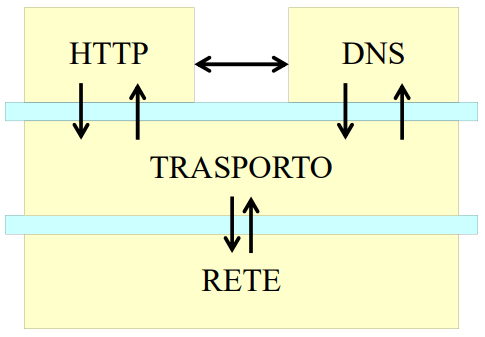
\includegraphics[scale=0.7]{schemadns.png}
\columnbreak

Il DNS è un meccanismo che deve:
\begin{list}{}{}
\item \textbf{Specificare la sintassi} dei nomi \textbf{e le regole} per gestirli
\item \textbf{Consentire la conversione} nomi $\rightarrow$ indirizzi e viceversa
\end{list}

Il DNS è costituito essenzialmente da:
\begin{list}{}{}
\item \textbf{Schema di assegnazione dei nomi}, gerarchico e basato su domini
\item \textbf{Database distribuito} contenente i \textbf{nomi} e le \textbf{corrispondenze} con gli indirizzi
\item \textbf{Protocollo per la distribuzione} delle informazioni sui nomi \textbf{tra i vari name server}
\end{list}
\end{multicols}
\pagebreak
\subsection{Servizi}
I servizi offerti dal DNS sono molteplici:
\begin{list}{}{}
\item \textbf{Risoluzione} di nomi di alto livello (\textbf{hostname}) in indirizzi IP
\item \textbf{Host aliasing}: un host può avere più nomi, solitamente il nome canonico + sinonimi.\\
Es. \texttt{realy1.west-coast.enterprise} può avere due alias \texttt{enterprise.com} e \texttt{www.enterprise.com}.
\item \textbf{Mail Server aliasing}: ci possono essere domain name identici per mail server e web server
\item \textbf{Distribuzione del carico} tra vari server replicati.\\
Ad un hostname canonico possono corrispondere diversi indirizzi IP. La lista di indirizzi viene ordinata in modo diverso in ogni risposta alla richiesta di risoluzione del nome, così che ogni server replicato possa essere scelto con uguale probabilità, distribuendo così efficientemente le richieste.
\end{list}
\subsection{Spazio dei nomi}
Dato che internet è una rete di proporzioni enormi, si presentano i problemi di \textbf{identificazione delle macchine} e \textbf{instradamento dei pacchetti}. si adotta un \textbf{approccio stratificato} poiché è un sistema complesso.\\
\subsubsection{Indirizzi} In internet esistono più indirizzi
\begin{list}{}{}
\item Indirizzi \textbf{MAC}, quello della scheda di rete.\\Solitamente prefissato
\item Indirizzo \textbf{di rete} (\textbf{IP})\\Es. \texttt{150.217.8.21}\\Assegnato dal gestore di rete in base al tipo di rete a cui si appartiene (classe di sottorete)
\item Indirizzo \textbf{di trasporto}\\Coppia $<$\texttt{indirizzo IP}, \texttt{porta}$>$\\La porta è scelta a livello applicativo con regole appropriate
\item Indirizzo \textbf{alfanumerico}\\Es \texttt{medialab.det.unifi.it}\\Libero, basta che sia mappato in un NameServer
\end{list}
\subsubsection{Nomi}
Lo \textbf{spazio dei nomi} deve permettere di \textbf{identificare in modo univoco} un host.
\begin{list}{}{}
\item \textbf{Struttura flat}: sequenza di caratteri senza alcuna ulteriore struttura. Poco applicabile.
\item \textbf{Struttura gerarchica}: un nome è \textbf{costituito da diverse parti}.\\Requisiti per la partizione dello spazio dei nomi:
\begin{list}{}{}
\item \textbf{Conversione efficiente}
\item \textbf{Controllo decentralizzato} dell'assegnazione dei nomi.\\Delega dell'autorità per le varie parti dello spazio dei nomi e \textbf{distribuzione della responsabilità} della conversione tra nomi e indirizzi
\end{list}
Vantaggi e svantaggi
\begin{list}{}{}
\item -- Minore velocità
\item + Maggiore flessibilità
\item + Riconfigurazione più veloce
\item + Possibilità di aggiornamenti decentrati
\end{list}
\end{list}
\pagebreak
\paragraph{Nomi di dominio} Spazio dei nomi con \textbf{struttura gerarchica}. I nomi hanno una \textbf{struttura ad albero} con un numero di livelli variabile. \textbf{Ogni nodo definisce un livello gerarchico} ed è individuato da un'\textbf{etichetta} (max 63 caratteri). Alla radice è associata un'etichetta vuota.\\
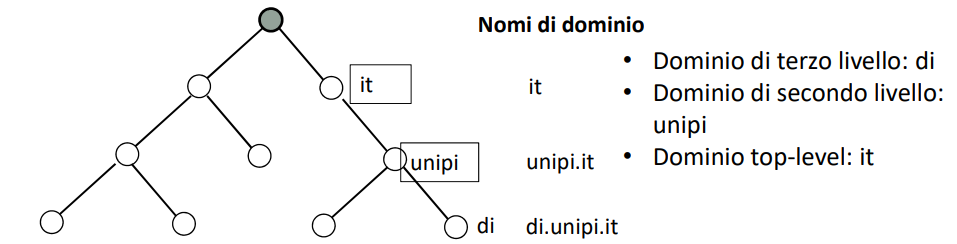
\includegraphics[scale=0.7]{nomidominio.png}\\
Ogni nodo dell'albero ha un nome di dominio, ovvero una \textbf{sequenza di etichette separate da punti} ovvero il cammino foglia $\rightarrow$ radice.
\subparagraph{Dominio} Sottoalbero nello spazio di nomi di dominio che viene identificato dal nome di dominio del nodo in cima al sottoalbero.\\Può essere suddiviso in ulteriori domini, detti \textbf{sottodomini}.
\paragraph{In Internet} Su internet i nomi gerarchici delle macchine sono \textbf{assegnati in base alla struttura delle organizzazioni} che ottengono l'autorità per porzioni dello spazio dei nomi. La struttura gerarchica permette \textbf{autonomia nella scelta dei nomi all'interno di un dominio} perché l'univocità è comunque garantita.\\
Ad es. \texttt{\textbf{server1}.di.unipi.it} e \texttt{\textbf{server1}.cs.cornell.edu} sono due nomi diversi.\\\\
Internet è divisa in \textbf{diverse centinaia di domini} ognuno dei quali \textbf{partizionato in sottodomini} e così via.
\begin{center}
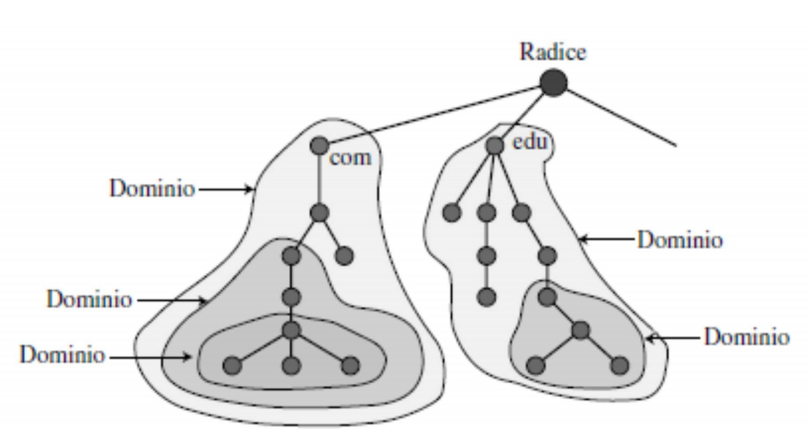
\includegraphics[scale=0.7]{domini.png}
\end{center}
\pagebreak
\subsubsection{Top-Level Domains}
\textbf{Internet Assigned Number Authority} IANA -- \texttt{iana.org}
\begin{list}{}{}
\item \texttt{com} Organizzazioni commerciali
\item \texttt{edu} Istituti d'istruzione (università, scuole\ldots)
\item \texttt{mil} Gruppi militari
\item \texttt{gov} Istituzioni governative
\item \texttt{net} Principali centri di supporto alla rete
\item \texttt{org} Organizzazioni diverse dalle precedenti
\item Codici geografici, schema geografico per nazioni\\Es. \texttt{ir}, \texttt{uk}, \texttt{us}, \texttt{fr}\ldots
\end{list}
\begin{center}
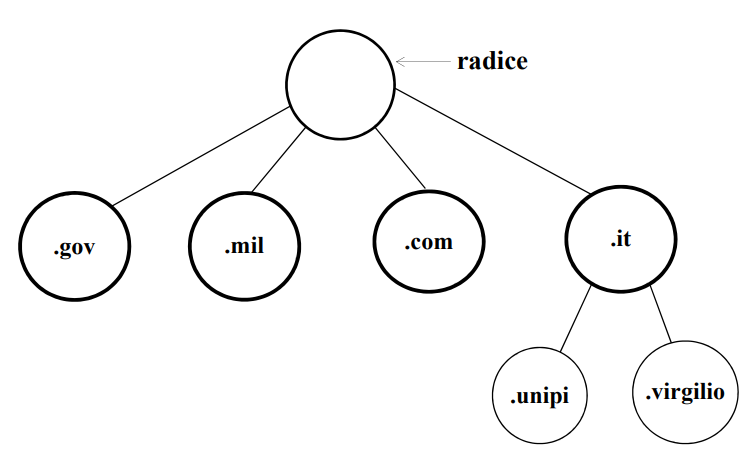
\includegraphics[scale=0.7]{gerarchianomidominio.png}
\end{center}
\subsubsection{Struttura di un nome alfanumerico}
\begin{center}
\texttt{mmedia5.di.unipi.it}
\end{center}
\begin{list}{}{}
\item \texttt{mmedia5} nome locale della macchina (etichetta \textbf{più specifica})
\item \texttt{di.unipi.it} nome del dominio (\texttt{.it} è l'etichetta \textbf{meno specifica})
\item La parte dominio \textbf{può essere ulteriormente suddivisa}, creando così una \textbf{struttura logica gerarchica}\\(\texttt{di} nome locale, \texttt{unipi.it} dominio e così via\ldots)
\end{list}
\pagebreak
\subsection{Conversione}
\paragraph{Indirizzi IP} Gli indirizzi IP sono \textbf{interi a 32bit}. Vengono rappresentati nella \textbf{Decimal Dotted Notation} che divide l'indirizzo IP in 4 \textbf{ottetti}, ovvero 4 gruppi di 8bit. Ad es. \texttt{150.217.8.21}.
\subparagraph{Gerarchia} L'indirizzo IP è strutturato in una gerarchia a due soli livelli.
\paragraph{Indirizzi alfanumerici} Gli indirizzi alfanumerici sono del tipo "\texttt{medialab.di.unipi.it}", sono \textbf{logici}, \textbf{gerarchici} e \textbf{NON indicano in assoluto la locazione geografica} di un host.\\
Vengono \textbf{convertiti da un Domain Name Server in un indirizzo IP}, eventualmente usando un sistema ricorsivo di ricerca.
\paragraph{Database DNS} Il database DNS è \textbf{distribuito} ed implementato in una gerarchia di più name servers.
\paragraph{Protocollo} Il protocollo per la \textbf{risoluzione dei nomi alfanumberici in indirizzi IP} è dello \textbf{strato applicativo}.
\subparagraph{NB} Una funzione fondamentale di internet è implementata come protocollo dello strato applicazione $\rightarrow$ una parte della complessità della rete è \textbf{gestita alle estremità} della rete stessa.
\subsubsection{Name Servers}
Un \textbf{Name Server} è un \textbf{programma che gestisce la conversione da nome di dominio ad indirizzo IP}. I Name Server sono strutturati gerarchicamente.
\begin{center}
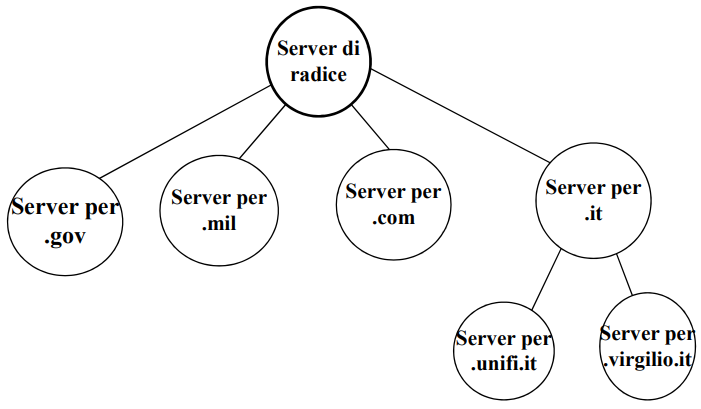
\includegraphics[scale=0.75]{strutturanameservers.png}
\end{center}
Spesso i DNS sono \textbf{accorpati} e \textbf{duplicati} (\textbf{sicurezza}). Inoltre per diminuire il traffico di rete ed il carico dei DNS, ogni server usa \textbf{una cache per le ultime richieste espletate}.
\begin{multicols}{2}
\paragraph{Informazioni} Le informazioni sui domini sono ripartite su più server
\paragraph{Zona} Una zona è una \textbf{regione di cui è responsabile un name server}, tipicamente una parte contigua dell'albero. Zona e dominio non necessariamente coincidono.\\
Il server \textbf{immagazzina le informazioni relative alla propria zona}, inclusi i riferimenti ai server dei domini di livello inferiore.
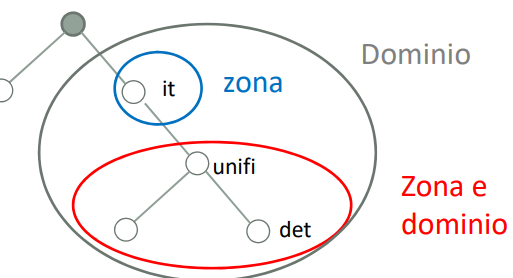
\includegraphics[scale=0.7]{zonadominio.png}
\end{multicols}
\pagebreak

\end{document}